\documentclass[11pt,a4paper,faculty=we,language=en,doctype=report]{cls/ugent-doc}

% Optional: margins and spacing
%-------------------------------
% Uncomment and adjust to change the default values set by the template
% Note: the defaults are suggested values by Ghent University
%\geometry{bottom=2.5cm,top=2.5cm,left=3cm,right=2cm} 
%\renewcommand{\baselinestretch}{1.15} % line spacing
\setlength{\headheight}{13.59999pt}

% Font
%------
%\usepackage[T1]{fontenc}
\usepackage[utf8]{inputenc} % allows non-ascii input characters
\usepackage{tikz-feynman}
% Comment or remove the two lines below to use the default Computer Modern font
%\usepackage{libertine}
%\usepackage{libertinust1math}

\usepackage[sc]{mathpazo} %font or smth
\linespread{1.05}
\usepackage{microtype}

\usepackage{fancyhdr} % Headers and footers
\pagestyle{fancy} % All pages have headers and footers e.g contents above contents (except new ones)
\usepackage[Rejne]{fncychap} %fancy chapters
%options for chapters: Sonny, Lenny, Glenn, Conny, Rejne, Bjarne, Bjornstrup

% NOTE: because the UGent font Panno is proprietary, it is not possible to use it
% in Overleaf. But UGent does not suggest to use Panno for documents (or maybe only for
% the titlepage). For the body, the UGent suggestion is to use a good serif font (for
% LaTeX this could be libertine or Computer Modern).
\usepackage{slashed}
\usepackage{braket}

% Proper word splitting
%-----------------------
\usepackage[english]{babel} 

% Mathematics
%-------------
\usepackage{amsmath}
\usepackage{amsfonts}
\usepackage{mathrsfs}
% Figures
%---------
%\usepackage{graphicx} % optional: the package is already loaded by the template
\graphicspath{{./figures/}}
\usepackage{copyrightbox}
% Bibliography settings
%-----------------------
\usepackage{cite}

% Hyperreferences
%-----------------
\usepackage[colorlinks=true, allcolors=ugentblue]{hyperref}

% Whitespace between paragraphs and no indentation
%--------------------------------------------------
\usepackage[parfill]{parskip} 

% Input for title page
%----------------------

% The title
\thetitle{Radio detection of high energy neutrinos in the Greenland icecap}
\thesubtitle{Arthur Adriaens}

%% Note: a stricter UGent style could be achieved with, e.g.:
\usepackage{ulem} % for colored underline
\renewcommand{\ULthickness}{2pt} % adjust thickness of underline
\thetitle{\uline{\color{ugentblue}Radio detection of high energy neutrinos in the Greenland icecap}}
% Note: do not forget to reset the \ULthickness to 1pt after invoking \maketitle
% (otherwise all underlines in the rest of your document will be too thick):
%\renewcommand{\ULthickness}{1pt}

% The first (top) infobox at bottom of titlepage
\infoboxa{\bfseries\large Department of Physics and Astronomy}

% The second infobox at bottom of titlepage
\infoboxb{Promotor: 
\begin{tabular}[t]{ll}
    Prof. dr. Dirk Ryckbosch & Dirk.Ryckbosch@ugent.be\\ % note syntax 'short space'
\end{tabular}
}

% The third infobox at bottom of titlepage
\infoboxc{Accompanist: 
\begin{tabular}[t]{ll}
    Bob Oeyen &  Bob.Oeyen@ugent.be\\
\end{tabular}
}

% The last (bottom) infobox at bottom of titlepage
\infoboxd{Academic year: 2022--2023} % note dash, not hyphen
\infoboxd{Master’s dissertation submitted in partial fulfilment of the requirements for the degree of master in Physics and Astronomy}

\begin{document}

% =====================================================================
% Cover
% =====================================================================

% ------------ TITLE PAGE ---------
\maketitle
\renewcommand{\ULthickness}{1pt}

% =====================================================================
% Front matter
% =====================================================================

% ------------ TABLE OF CONTENTS ---------
{\hypersetup{hidelinks}\tableofcontents} % hide link color in toc
\newpage


% =====================================================================
% Main matter
% =====================================================================
\chapter{Foreword}
\section{Abstract: English}
The Radio Neutrino Observatory - RNO-G - is under construction at Summit Station in Greenland to search for neutrinos of several PeV energy up to the Eev range. It's a mid-scale, discovery phase, extremely high-energy neutrino telescope that will probe the astrophysical neutrino flux at energies beyond the reach of IceCube.
More particularly if will make it possible to reach the next major milestone in astroparticle physics: the discovery of cosmogenic neutrinos.
\vspace{0.5cm}
All simulations carried out within this work were made with the three programs 
\begin{itemize}
	\item NuRadioMC
	\item radiotools
	\item RadioPropa
\end{itemize}
whom are free to download on \href{https://github.com/nu-radio}{github}
\section{Abstract: Nederlands}
% =====================================================================
\chapter{Background: Neutrinos}
\section{Electroweak interaction}
\begin{align*}
  \mathcal{L}_{SM} &= -\frac{1}{4}F_{\mu\nu}F^{\mu\nu}\\
                   & + i\bar{\psi}\slashed{\mathcal{D}}\psi + h.c\\
                   & + \psi_iy_{ij}\psi_j\phi + h.c\\
                   &+|\mathcal{D}_\mu\phi|^2 - V(\phi)
\end{align*}
Above we see the standard model lagrangian density, consisting of the following parts: at the top the Generalized maxwell lagrangian,
the second line being the generlaized lorentz force, the third line the yukawa couplings and the last line responsible for
the mass of the W\&Z bozons via the Brout Englert Higgs mechanism. We'll mostly concern ourselves with 
the second part.
\subsection{History}
Fermi realised a quantitatively good local field theory for the $\beta$-decay in 1934 based on the idea of the following
interaction:
\begin{equation}
	n \rightarrow p + e^- + \bar{\nu} \label{eqn:neutron decay}
\end{equation}
i.e
\begin{figure}[h!]
	\centering
	\begin{tikzpicture}
	\begin{feynman}
	\vertex (a0){n};
	\vertex[right=2cm of a0] (ah) ;
	\vertex[right=4cm of a0] (a1) {$\nu$};
	\vertex[above=4cm of a0] (a3){p};
	\vertex[right=4cm of a3] (a2){$e^-$};
	\vertex[above=2cm of ah] (am);
	\diagram* {
		{[edges=fermion]
			(a0) -- (am) -- (a3)
		},
		{[edges=fermion]
			(a1) -- (am) -- (a2)
		}
	};
	\end{feynman}
	\end{tikzpicture}
\end{figure}\\
This 4-fermion interaction is however not renormalizable, meaning that it will be incorrect for sufficiently high
energies. As the lagrangian density would look like
\begin{equation}
	\mathcal{L}^F_{int} = -G_F (\bar{\psi}_p\gamma_\mu \psi_n) (\bar{\psi}_e\gamma^\mu\psi_\nu) + h.c
\end{equation}\\
And indeed, from dimensionality analysis we see that, as $[\psi]=[L]^{-3/2}$, we get that from $[\mathcal{L}_{int}] = [L]^{-4}$, $[G_F] = [L]^2 = [\Lambda]^{-2}$

This interaction lagrangian density also doens't explain how this weak interaction violates parity, as was observed in the $\tau-\theta$ puzzle where it has become apparent that the weak interaction only couples
to the left handed part of lepton- and baryon fields. Everything was finally explained using
the V-A model, which we'll get to shortly.

\subsection{Chiral gauge theories}
Let's first give a quick example on how parity can be broken in a gauge theory; let's define the operators
\begin{equation}
	P_R = \frac{1}{2}(1+\gamma_5)\quad P_L = \frac{1}{2}(1-\gamma_5)
\end{equation}
with
\begin{equation}
	\gamma_5 = i\gamma_0\gamma_1\gamma_2\gamma_3
\end{equation}
And with this defining 
\begin{equation}
	\psi_R := P_R\psi \quad \psi_L := P_L\psi
\end{equation}
Now starting from the simple kinetic lagrangian density:
\begin{equation}
  \mathcal{L} = i\bar{\psi}\slashed{\partial}\psi - m\bar{\psi}\psi
\end{equation}
We can re-write this as follows:
\begin{equation}
  \mathcal{L} = i\bar{\psi}_R\slashed{\partial}\psi_R + i\bar{\psi}_L\slashed{\partial}\psi_L - m\bar{\psi}_R\psi_L - m\bar{\psi}_L\psi_R
\end{equation}
Now we wish to have gauge invariance over the whole lagrangian density, 
i.e having
\begin{align}
  &\psi_R(x) \rightarrow \psi_R'(x) = e^{iq_R f(x)}\psi_R(x)\\
  &\psi_L(x) \rightarrow \psi_L'(x) = e^{iq_L f(x)}\psi_L(x)
\end{align}
Now in the maxwellian term of the standard model, as 
\begin{equation}
  F_{\mu\nu} = \partial_\mu A_\nu - \partial_\mu A_\nu
\end{equation}
The A field has a gauge transform of the form
\begin{equation}
	A_\mu(x) \rightarrow A_\mu'(x) = A_\mu(x) - \partial_\mu f(x) \label{eqn:U(1) gauge transform}
\end{equation}
Thus if we define the covariant derivatives
\begin{align}
  \mathcal{D}_\mu\psi_R &= \partial_\mu\psi_R + iq_RA_\mu\psi_R\\
  \mathcal{D}_\mu\psi_L &= \partial_\mu\psi_L + iq_LA_\mu\psi_L
\end{align}
We see that our lagrangian density
\begin{equation}
  \mathcal{L} = i\bar{\psi}_R\slashed{\mathcal{D}}\psi_R + i\bar{\psi}_L\slashed{\mathcal{D}}\psi_L
\end{equation}
Is gauge invariant. If you write this out you get
\begin{equation}
  i\bar{\psi}\slashed{\partial}\psi - \frac{q_R + q_L}{2}\bar{\psi}\slashed{A}\psi - \frac{q_R - q_L}{2}\bar{\psi}\slashed{A}\gamma_5\psi
\end{equation}
The rightmost term is a pseudoscalar, we thus see that this system breaks
parity invariance if $ q_L \neq q_R$. This is a crude form of the V-A theory.

\subsection{$SU(2) \rightarrow SU(2)_L \times U(1)_Y$}
We'll now quickly derive and discuss the weak interaction
looking at a 2x2 constant $\mathbb{C}$ transformation
\begin{align}
	\Psi(x) &\rightarrow M\Psi(x)\\
\bar{\Psi}(x) &\rightarrow \bar{\Psi}(x)M^\dagger
\end{align}
We want the lagrangian density to be gauge invariant meaning that we wish them to obey
\begin{equation}
	M^\dagger M = \mathbb{1}_{2x2}
\end{equation}
i.e we want them to be unitary, aside from this we also choose $det(M)=1$ restricting ourselves to
the special unitary 2D matrices (the SU(2) group), we get that if we take a look at the kinetic lagrangian
density:
\begin{equation}
	\mathcal{L} = i\bar{\Psi}\slashed{\partial}\Psi - m\bar{\Psi}\Psi
\end{equation}
requiring invariance under the previously mentioned transformation, calculating we have that:
\begin{equation}
	\partial_\mu \Psi \rightarrow \partial_\mu(M \Psi) = M(\partial_\mu \Psi + M^{-1}\partial_\mu M \Psi)
\end{equation}
Now
\begin{equation}
	(M^{-1}\partial_\mu M)^\dagger = \partial_\mu M^\dagger (M^{-1})^\dagger = \partial_\mu M^{-1}M
\end{equation}
Due to them being from the SU(2) group, now as $M^{-1}M = \mathbb{1}_{2x2}$:
\begin{equation}
	\partial_\mu (M^{-1}M) = 0 \implies \partial_\mu M^{-1}M = -M^{-1}\partial_\mu M
\end{equation}
i.e $M^{-1}\partial_\mu M$  is anti-hermitian, now 
\begin{align}
	\frac{\delta det(M)}{det(M)} &= tr(M^{-1}\delta M)\\
	\frac{\partial_\mu det(M)}{det(M)} &= tr(M^{-1}\delta M)
\end{align}
The left side is zero as $det(M)=0$, thus $M^{-1}\partial_\mu M$ is traceless and anti-hermitian,
meaning that to make the lagrangian density gauge invariant under $SU(2)$, we can define
the covariant derivative
\begin{equation}
	\mathcal{D}_\mu\Psi = \partial_\mu\Psi + igW_\mu\Psi
\end{equation}
With $W_\mu$ a traceless hermitian 2x2 matrix of gauge fields and $g\in\mathbb{R}$ a coupling constant.
Now as is well know the complete basis of 2x2 hermitian traceless matrices are the Pauli matrices
\begin{equation}
	\sigma_1 = \left(\begin{matrix}0&1\\1&0\end{matrix}\right)\quad \sigma_2 = \left(\begin{matrix}0&-i\\i&0\end{matrix}\right)\quad \sigma_3 = \left(\begin{matrix}1&0\\0&-1\end{matrix}\right)
\end{equation}
meaning we can construct the gauge fields as
\begin{equation}
	W_\mu = \frac{1}{2}\sum^3_{a=1} W_\mu^a(x) \sigma_a = \frac{1}{2}\left(\begin{matrix}W_\mu^3&W_\mu^1-iW_\mu^2\\W_\mu^1+iW_\mu^2&-W_\mu^3\end{matrix}\right)
\end{equation}
The lagrangian density then becomes
\begin{equation}
	\mathcal{L} = i\bar{\Psi}\slashed{\partial}\Psi - m\bar{\Psi}\Psi - g\bar{\Psi}\slashed{W}\Psi := \mathcal{L}_0 + \mathcal{L}_I
\end{equation}
I.e we get an extra interaction term.
Now defining 
\begin{align}
	W_\mu &:= \frac{1}{\sqrt{2}}(W_\mu^1 - iW_\mu^2)\\
	W_\mu^\dagger &:= \frac{1}{\sqrt{2}}(W_\mu^1 + iW_\mu^2)
\end{align}
The interaction lagrangian density becomes 
\begin{align}
	\mathcal{L}_I &= -\frac{g}{2}(\bar{\psi}_1,\bar{\psi}_2)\left(\begin{matrix}\slashed{W}^3&\sqrt{2}\slashed{W}\\\sqrt{2}\slashed{W}^\dagger&-\slashed{W}^3\end{matrix}\right)\left(\begin{matrix}\psi_1\\\psi_2\end{matrix}\right)\\
		      &= -\frac{g}{2}\bar{\psi}_1\slashed{W}^3\psi_1 + \frac{g}{2}\bar{\psi}_2\slashed{W}^3\psi_2\\
		      &\qquad-\frac{g}{\sqrt{2}}\bar{\psi}_1\slashed{W}\psi_2 + \frac{g}{\sqrt{2}}\bar{\psi}_2\slashed{W}^\dagger\psi_1
\end{align}
I.e a flavour changing part and a non-flavour changing part. If we now set up this system with the vector
\begin{equation}
	\Psi_\ell^L = \left(\begin{matrix}\nu_l^L\\\ell^L\end{matrix}\right)
\end{equation}
With also a U(1) transformation:
\begin{equation}
	\Psi_\ell^L \rightarrow \Psi_\ell^{L'}(x) = M(x) e^{ig'q\beta(x)}\Psi_\ell^L(x)
\end{equation}
Introducing the U(1) gauge field $B_\mu$ that transforms as in equation \ref{eqn:U(1) gauge transform}
we see that the covariant derivative needs to be defined as 
\begin{equation}
	\mathcal{D}_\mu \Psi_\ell^L = \partial_\mu \Psi_\ell^L + ig\hat{W}_\mu \Psi_\ell^L + ig'qB_\mu\Psi_\ell^L
\end{equation}
Yielding an interaction lagrange density of the form
\begin{equation}
	\mathcal{L}_I = \sum_\ell - g\bar{\Psi}^L_\ell \hat{\slashed{W}}\Psi^L_\ell - g'q\bar{\Psi}_\ell^L\slashed{B}\Psi^L_\ell
\end{equation}
And after introducing the weak mixing angle (Glashow):
\begin{align}
	W_\mu^3 &= \sin(\theta_W)A_\mu + \cos{(\theta_W)}Z_\mu\\
	B_\mu &= \cos{(\theta_W)}A_\mu + \sin{(\theta_W)}Z_\mu
\end{align}
We can go ahead and find our interaction lagrangian density for the
photon field $A_\mu$, the W-boson field $W_\mu$ and the Z-boson field $Z_\mu$.
Then an analogous analysis can be done for the quark sector and we have fully 
developed the electroweak theory\footnote{note that this can be further generalized to arrive at
cubic and quartic couplings e.g WWWW couplings which I won't go into here as it isn't relevant 
for this discussion, the symmetry breaking needed to give mass to the bosons also won't be 
discussed}
, thus in part finding the possible interactions that can happen with neutrinos:
\begin{equation}
	\mathcal{L}_{I}^{\nu} =\sum_l-\frac{g}{2 \sqrt{2}} \bar{\nu}_l \slashed{W}\left(1-\gamma_5\right)l - \frac{g}{2 \sqrt{2}} \bar{l}\slashed{W}^\dagger\left(1-\gamma_5\right) \nu_l
\end{equation}
i.e
\begin{figure}[h!]
	\begin{minipage}{0.49\textwidth}
	\centering
	\begin{tikzpicture}
	\begin{feynman}
	\vertex (a0){l};
	\vertex[right=2cm of a0] (am) ;
	\vertex[right=2cm of am] (a1) {$\nu_l$};
	\vertex[above=2cm of am] (ah) {W};
	\diagram* {
		{[edges=fermion]
			(a0) -- (am) -- (a1)
		},
		{[edges=boson]
			(am) -- (ah)
		}
	};
	\end{feynman}
	\end{tikzpicture}
	\end{minipage}
	\begin{minipage}{0.49\textwidth}
	\centering
	\begin{tikzpicture}
	\begin{feynman}
	\vertex (a0){$\bar{l}$};
	\vertex[right=2cm of a0] (am) ;
	\vertex[right=2cm of am] (a1) {$\bar{\nu}_l$};
	\vertex[above=2cm of am] (ah) {$W^\dagger$};
	\diagram* {
		{[edges=fermion]
			(a1) -- (am) -- (a0)
		},
		{[edges=boson]
			(am) -- (ah)
		}
	};
	\end{feynman}
	\end{tikzpicture}
	\end{minipage}
\end{figure}\\
%\subsection{Majorana}
\section{Do neutrinos have mass?}
Neutrinos get produced through the following ways in the nucleus of our star:\\
$\bold{pp-cycle}$
\begin{align}
	\mathrm{p} + \mathrm{p} &\rightarrow \mathrm{D} + e^+ + \nu_e\\
	\mathrm{D} + \mathrm{p} &\rightarrow {}^3\mathrm{He} + \gamma\\
	{}^3\mathrm{He} + {}^3\mathrm{He} &\rightarrow {}^4\mathrm{He} + \mathrm{p} + \mathrm{p}
\end{align}\\
$\bold{boron-cycle}$
\begin{align}
{ }^4 \mathrm{He}+{ }^3 \mathrm{He} & \rightarrow{ }^7 \mathrm{Be}+\gamma \\
{ }^7 \mathrm{Be}+p & \rightarrow { }^8\mathrm{B} + \gamma \\
{ }^8 \mathrm{B} & \rightarrow{ }^8 \mathrm{Be}^*+e^{+}+\nu_e \\
{ }^8 \mathrm{Be}^* & \rightarrow{ }^4 \mathrm{He}+{ }^4 \mathrm{He}
\end{align}\\
$\bold{Be-capture}$
\begin{align}
	^7\mathrm{Be} + e^- \rightarrow {}^7\mathrm{Li} + \nu_e
\end{align}
$\bold{pep}$
\begin{align}
	\mathrm{p} + e^- + \mathrm{p} \rightarrow \mathrm{D} + \nu_e
\end{align}\\
Now with this and some information about the sun like the pressure and mass, 
the so-called "standard solar model" was
made. This model predicted a certain amount of neutrinos to be hitting the earth from the previously
mentioned thermonuclear fusion, it was however 3 times higher than the observed amount of neutrinos back
at our planet. Through various experiments it became apparent that this was due to the various kind of
neutrinos oscillating into each other, i.e 2/3 of the original electron 
neutrinos had oscillated into mu and tau neutrinos
but for them to oscillate into eachother, they require mass
\subsection{neutrino oscillations}
Let's only discuss this in 2D (this can easily be extended to 3D but we wish to be 
concise and only show the principle), define the mass-eigenstates as 
\begin{equation}
	\ket{\nu_i(t)} = \ket{\nu_i}\exp\{i(\mathbf{p}_i\cdot\mathbf{x} - E_i t)\} = \ket{\nu_i}e^{-i\phi}
\end{equation}
Now let's say these are related to the *originals* as:
\begin{equation}
	\left(\begin{matrix}\nu_e\\\nu_\mu\end{matrix}\right)=\left(\begin{matrix}\cos{\theta}&\sin{\theta}\\-\sin{\theta}&\cos{\theta}\end{matrix}\right)\left(\begin{matrix}\nu_1\\\nu_2\end{matrix}\right)
\end{equation}
Assume at $t=0$ pure $\nu_e$ (starting at the sun core):
\begin{equation}
	\ket{\psi(0)} = cos{\theta} \ket{\nu_1} + \sin{\theta}\ket{\nu_2}
\end{equation}
At time $T$, at distance $L$
\begin{align}
	\ket{\psi(L, T)} &= \cos{\theta} \ket{\nu_1}e^{-i \phi_1}+\sin{\theta}\ket{\nu_2}e^{-i \phi_2}\\
			 &= (e^{-i\phi_1}\cos^2{\theta} + e^{-i\phi_2}\sin^2{\theta})\ket{\nu_e} 
			 - (e^{-i\phi_1} - e^{-\phi_2})\cos{\theta}\sin{\theta}\ket{\nu_\mu}
\end{align}
\begin{align}
&\quad=e^{-i \phi_1} {\left[\left(\cos ^2 \theta+e^{i \Delta \phi_{12}} \sin ^2 \theta\right) \mid \nu_e>\right.} \\
&\qquad\left.-\left(1-e^{i \Delta \phi_{12}}\right) \cos \theta \sin \theta \mid \nu_\mu>\right]\\
&\quad:=c_e\ket{\nu_e} c_\mu\ket{\nu_\mu}
\end{align}
With
\begin{equation}
	\Delta \phi_{12}=\left(E_1-E_2\right) T-\left(p_1-p_2\right) L
\end{equation}
So the transition probability is
\begin{equation}
	P(\nu_e\rightarrow\nu_\mu) = |\braket{\nu_\mu|\psi(L,T)}|^2 = c_\mu c_\mu^* = \sin ^2(2 \theta) \sin ^2\left(\frac{\Delta \phi_{12}}{2}\right)
\end{equation}
If you then proceed to do a full wave-packet propagation calculation you'll find
\begin{equation}
	\Delta \phi_{12} \approx \frac{m_1^2 - m_2^2}{2p}L
\end{equation}
I.e not only mass but difference in mass of the eigenstates is a requirement for oscillations to occur.
In general
\begin{equation}
	\ket{\nu_\alpha} = \sum_iU_{\alpha i} \ket{\nu_i}
\end{equation}
With $U_{\alpha i}$ e.g the Pontecorvo-Maki-Nakagawa-Sakata (PMNS) matrix. 
This phenomenon has been observed e.g from the descrepency from the observed
and expected neutrino events coming from a nuclear reactor \cite{Eguchi_2003}.
Now the question remains, how do neutrinos get their mass (theoretically)?
\subsection{See-saw mechanism}
Given a spinor $\psi$ with the following Lagrange density:
\begin{equation}
	\mathcal{L} = i\bar{\psi}\slashed{\partial}\psi - m\bar{\psi}\psi - \frac{M}{2} (\bar{\psi}_R\psi_{Rc} + \bar{\psi}_{Rc}\psi_R)
\end{equation}
We can re-write this Lagrangian in terms of
\begin{align}
	\chi &:= \frac{1}{\sqrt{2}} (\psi_R + \psi_{Rc})\\
	\omega &:= \frac{1}{\sqrt{2}} (\psi_L + \psi_{Lc})
\end{align}
by first identifying that
\begin{equation}
	- \frac{M}{2} (\bar{\psi}_R\psi_{Rc} + \bar{\psi}_{Rc}\psi_R)
\end{equation}
is equal to
\begin{equation}
	-M\bar{\chi} \chi = -\frac{M}{2} (\bar{\psi}_R + \bar{\psi}_{Rc}) (\psi_R + \psi_{Rc}) = -\frac{M}{2} (\bar{\psi}_R\psi_{Rc} + \bar{\psi}_{Rc}\psi_R)
\end{equation}
Where we've used
\begin{equation}
	\bar{\psi}_R\psi_{R} \equiv \psi_R^\dagger\gamma^0\psi_{R} \equiv P_R\psi^\dagger\gamma^0P_R\psi = P_RP_L\psi^\dagger\gamma^0\psi = 0
\end{equation}
And next that in
\begin{equation}
	i\bar{\psi}\slashed{\partial}\psi - m\bar{\psi}\psi = i\bar{\psi}_R\slashed{\partial}\psi_{R} + i\bar{\psi}_L\slashed{\partial}\psi_{L} - m\bar{\psi}_R\psi_{L} - m\bar{\psi}_L\psi_{R}
\end{equation}
We can identify that
\begin{align}
	\bar{\chi}\slashed{\partial}\chi &= \frac{1}{2}(\bar{\psi}_R\slashed{\partial}\psi_{R} + \bar{\psi}_{Rc}\slashed{\partial}\psi_{Rc}) = \bar{\psi}_R \slashed{\partial} \psi_{R}\\
	\bar{\omega}\slashed{\partial}\omega &= \bar{\psi}_L \slashed{\partial} \psi_{L}
\end{align}
Where we've done an integration by parts and used $\bar{\psi}_c\gamma_\mu\chi_c = -\bar{\chi}\gamma_\mu\psi$. We thus get:
\begin{equation}
	\mathcal{L} = i\bar{\chi}\slashed{\partial}\chi +i\bar{\omega}\slashed{\partial}\omega - m\bar{\psi}_R\psi_{L} - m\bar{\psi}_L\psi_{R} -M\bar{\chi} \chi 
\end{equation}
And finally we notice that
\begin{align}
	\bar{\chi}\omega &= \frac{1}{2} \left(\bar{\psi}_R\psi_L + \bar{\psi}_R\psi_{Lc} + \bar{\psi}_{Rc}\psi_{L} + \bar{\psi}_{Rc}\psi_{Lc}\right)\\
	&=  \frac{1}{2} \left(\bar{\psi}_R\psi_L + \bar{\psi}_R\psi_{Lc} + \bar{\psi}_{Rc}\psi_{L} + \bar{\psi}_{L}\psi_{R}\right)\\
	\bar{\omega}\chi &= \frac{1}{2} \left(\bar{\psi}_L \psi_{R} + \bar{\psi}_{Lc}\psi_{R} + \bar{\psi}_L\psi_{Rc} + \bar{\psi}_{Lc}\psi_{Rc}\right)\\
	&= \frac{1}{2} \left(\bar{\psi}_L \psi_{R} + \bar{\psi}_{Lc}\psi_{R} + \bar{\psi}_L\psi_{Rc} + \bar{\psi}_{R}\psi_{L}\right)
\end{align}
As $\bar{\psi}_c\chi_c = \bar{\chi}\psi$. Summing these, we get:
\begin{align}
	\bar{\chi}\omega + \bar{\omega}\chi &= \bar{\psi}_L \psi_R + \bar{\psi}_R \psi_{L}\\
	&\quad + \frac{1}{2}\left(\bar{\psi}_R\psi_{Lc} + \bar{\psi}_{Rc} \psi_{L} + \bar{\psi}_{Lc}\psi_R + \bar{\psi}_L\psi_{Rc}\right)\\
	&= \bar{\psi}_L \psi_R + \bar{\psi}_R \psi_{L}
\end{align}
Where we've used the handedness flips a charge conjugation entails, at last we now have:
\begin{equation}
	\mathcal{L} = i\bar{\chi}\slashed{\partial}\chi +i\bar{\omega}\slashed{\partial}\omega - m(\bar{\chi}\omega + \bar{\omega}\chi) -M\bar{\chi} \chi 
\end{equation}
Now to determine the mass eigenstates we'll re-write this equation into the form
\begin{equation}
	\mathcal{L} = i\bar{\chi}\slashed{\partial}\chi +i\bar{\omega}\slashed{\partial}\omega 
	-\left(\begin{array}{cc}
		\bar{\chi} &\bar{\omega}
	\end{array}\right)\cdot
	\left(\begin{array}{cc}
		M & m \\
		m & 0
	\end{array}\right) \cdot \left(\begin{array}{c}
	\chi \\ \omega
\end{array}\right)
\end{equation}
lets now find the eigenvalues:
\begin{equation}
	\left| \begin{array}{cc}
		M-\lambda & m \\
		m & -\lambda
	\end{array} \right| = (\lambda-M)\lambda - m^2 = 0 \implies \lambda_\pm  = \frac{M\pm \sqrt{M^2 + 4m^2}}{2} \label{eigenvalues}
\end{equation}
i.e
\begin{equation}
	\lambda_\pm = \frac{M}{2}\left( 1 \pm \sqrt{1 + 4m^2/M^2}\right)
\end{equation}
Now we'll determine the eigenvectors:
\begin{equation}
\left[\begin{array}{cc}
	M-\lambda_\pm & m \\
	m & -\lambda_\pm
\end{array}\right] \left(\begin{array}{c}
x_\pm \\
y_\pm
\end{array}\right) = \vec{0}
\end{equation}
this gives
\begin{align}
	Mx_\pm - \lambda_\pm x_\pm + my_\pm &= 0\\
	m x_\pm - \lambda_\pm y_\pm &= 0 \implies \frac{m x_\pm}{\lambda_\pm} = y_\pm
\end{align}
inserting the second equation in the first we get:
\begin{align}
	Mx_\pm - \lambda_\pm x_\pm + m \frac{m x_\pm}{\lambda_\pm} = 0 &= M\lambda_\pm x_\pm - \lambda_\pm^2 x_\pm + m^2 x_\pm\\
	&= x_\pm(\lambda_\pm^2 -M\lambda_\pm + m^2)
\end{align}
which is true for every $x_\pm$ (see equation \ref{eigenvalues}) i.e we can freely choose $x_\pm$ so let's opt for $x_\pm^2 + y_\pm^2 = 1$:
\begin{align}
	x_\pm^2(1+\frac{m^2}{\lambda_\pm^2}) = 1 \implies x^2_\pm = \frac{1}{1+\frac{m^2}{\lambda_\pm^2}} \implies x_\pm &= \frac{\lambda_\pm}{\sqrt{\lambda_\pm^2 + m^2}}\\
	\& \quad y_\pm &= \frac{m}{\sqrt{\lambda_\pm^2 + m^2}}
\end{align}
And thus, summing up, we get the eigenvectors $\phi_\pm$ with eigenvalues $m_\pm$:
\begin{equation}
	\phi_\pm := \left(\begin{array}{c}
		x_\pm\\
		y_\pm
	\end{array}\right) = \left(\begin{array}{c}
		\frac{\lambda_\pm}{\sqrt{\lambda_\pm^2 + m^2}}\\
		\frac{m}{\sqrt{\lambda_\pm^2 + m^2}}
	\end{array}\right) \quad \text{ and }\quad m_\pm := \lambda_\pm =  \frac{M}{2}\left( 1 \pm \sqrt{1 + 4m^2/M^2}\right)
\end{equation}
Now we'll consider the limit $M \gg m$:
\begin{equation}
	m_\pm =  \frac{M}{2}\left( 1 \pm \sqrt{1 + 4m^2/M^2}\right) \approx \frac{M}{2}\left(1\pm1\pm\frac{2m^2}{M^2}\right)
\end{equation}
Which gives:
\begin{align}
	m_+ &\approx M\\
	m_- &\approx -\frac{m^2}{M}
\end{align}
and:
\begin{align}
	\phi_+&\approx \left(\begin{array}{c}
		\frac{M}{M}\\
		\frac{m}{M}
	\end{array}\right) = \left(\begin{array}{c}
	1\\
	m/M
	\end{array}\right)\\
	\phi_-&\approx \left(\begin{array}{c}
		-\frac{m}{M}\\
		\frac{m}{m}
	\end{array}\right) = \left(\begin{array}{c}
		-m/M\\
		1
	\end{array}\right)
\end{align}
i.e, in the $\chi,\omega$ basis:
\begin{align}
	m_+\approx M \quad &\text{with eigenstate} \quad \chi + \frac{m}{M}\omega\\
	m_-\approx -\frac{m^2}{M} \quad &\text{with eigenstate} \quad  \omega - \frac{m}{M}\chi\\
\end{align}
This is what's called the See-Saw mechanism, and gives a possible explanation for the
small mass of the neutrinos.  For a certain $m$ if we choose a big $M$ we'll
get a big $m_+$ and small $m_-$ (and vice versa). We also see that there's only
a very small mixing of states, i.e the $m_-$ mass state is almost purely
$\omega$ (and $m_+$ almost purely $\chi$). The parameter $m$ in the original
matrix is forbidden by electroweak gauge symmetry, and can only appear after
the symmetry has been spontaneous broken by a Higgs mechanism; for this reason
a good estimate of the order of $m$ is the vaccuum expectation energy:
$m\approx v = 246 \approx 10^2$GeV. In grand unified theories it's theorised
that $M\approx 10^{15}$GeV after symmetry breaking, using these values we get
\begin{align}
	m_- \approx 10^{-11}\text{GeV} \approx 10^{-2} \text{eV}
\end{align}
which seems \cite{neutrino-mass} to be a reasonable order of magnitude estimate for the observed neutrino
mass.
This mechanism would also lead to supermassive neutrinos, which are a possible dark matter
candidate.
\section{Why concern ourselves with neutrinos}
%The radio detection of neutrinos targets the energy range 10PeV to 100EeV\cite{Aguilar_2021} 
Neutrinos are ideal messengers to identify the UHE (Ultra High Energy) sources
in the universe. Unlike cosmic rays, which are deflected by magnetic fields and
interact with matter and radiation on their way to us, neutrinos point back to
sources and can reach Earth unperturbed from the most distant corners of the
universe.  Neutrinos can be generated in 2 ways: either they're generated in
interactions at the sources, termed \textit{astrophysical neutrinos}. Or
they're created through the interaction of ultra-high energy cosmic rays during
propagation with the cosmic microwave or other photon backgrounds termed
\textit{cosmogenic neutrinos}. 
Supernovae are a source for \textit{astrophysical neutrinos}:
\subsection{Supernovae}
A star starts its life as a ball of pure hydrogen, at the core due to the
gravitational pressure of the outside plasma fusion of hydrogen into deuterium
and helium happens, converting mass into energy. The pressure of this energy
counteracts the pressure of gravity and the star is stable.

When the hydrogen at the core runs out no more hydrogen can be fused and the
fusion of heavier elements starts, this can't keep going on however as at some
point the star starts to form the most stable element: iron.  It costs energy
to both make lighter elements than iron and heavier ones.  As the iron core
builds up the outside pressure from the core starts to decrease as no new
energy is released. This goes on until the inwards pressure becomes too large
and the electrons surrounding the iron core fuse with the protons, 
creating neutrons and neutrino's.

This last part happens in a split second, creating a very dense neutron star
and up to $10^{52}$ ultra-relativistic neutrinos, carrying up to 99\% of the
released energy [citation needed]. As the density has suddenly
increased so much there's a huge distance of pure vaccuum between the plasma
outer layer and the (now) neutron star, this plasma starts free-falling inwards 
whilst the neutrinos carrying tremendous amounts of energy start going outwards 
from the neutron stars core.

These then collide resulting in what we observe as a "supernova", wrongly
thought of by Kepler as being a "new (nova) star" rather being a violent death
of an old star.

Not all the neutrinos collide with matter of course as neutrinos rarely
interact, it's only because the incoming plasma is so dense and due to the
tremendous amount of neutrinos that collissions happen at all. The ones that
escape, however, will be visible on earth in our neutrino detectors, far before
the light escapes the exploding star.

Neutrino observatories are thus useful to know where to point our various
telescopes before the supernova is actually visible in the night sky.
\subsection{primordial neutrinos}
Aside from all the previously mentioned sources, there's also a less spectacular source of 
neutrinos: the neutrino version of the CMB.
We can estimate the temperature of the neutrinos who decoupled at the start of the universe, 
we can take a look at conservation of entropy \cite{Dodelson}
(...)
The entropy before and after decoupling are:
\begin{align}
	s(a_1) &= \frac{2\pi^2}{45}(2 + \frac{7}{8}(2+2+3+3))T_1^3\\
	&= \frac{2\pi^2}{45}\frac{86}{8}T_1^3\\
	s(a_2) &= \frac{2\pi^2}{45}(2T_\gamma^3 + \frac{7}{8}(6)T_\nu^3)\\
\end{align}
Conservation of entropy:
\begin{align}
	s(a_1)a_1^3 &= s(a_2)a_2^3\\
	\frac{86}{8}(T_1 a_1)^3 &= \left(2\left(\frac{T_\gamma}{T_\nu}\right)^3 + \frac{42}{8}\right)(T_\nu a_2)^3\\
	\frac{86}{8} &= 2\left(\frac{T_\gamma}{T_\nu}\right)^3 + \frac{42}{8}\\
	\frac{44}{16} &= \left(\frac{T_\gamma}{T_\nu}\right)^3\\
	\left(\frac{T_\gamma}{T_\nu}\right) &= \left(\frac{11}{4}\right)^{1/3}
\end{align}
i.e
\begin{equation}
	T_\nu = \left(\frac{4}{11}\right)^{1/3}T_\gamma
\end{equation}
\subsection{How do they fit into the full detector spectrum?}
The origin of the most energetic cosmic rays is still not conclusively
identified. One approach to solving this problem is \textit{multi-messenger
astrophysics}, where several types of cosmic particles are used to identify the
sources of these ultra-high energy cosmic rays (UHECRs). E.g we simultaneously
measure gravitational waves (gravitons?) with the Einstein telescope,
neutrino's with IceCube (or eventually RNO-G), photons with various telescopes
and muons with a muon detector.
\newpage
\chapter{Background: Radio detection}
For a particle shower to emit strong radio signals, two conditions have to be met:
\begin{itemize}
	\item There needs to be a speration of positive and negative charges in the shower front 
	\item The signals produced over the length of the shower profile need to overlap coherently.
\end{itemize}
The first item, seperation of positive and negative charges, can be caused by 2
mechanisms:\vspace{0.2cm}\\
The \textit{Askaryan} \cite{Askaryan} effect, also known as Askaryan
radiation. This is the phenomenon whereby a particle traveling faster than the
phase velocity of light in a dense dielectric (such as ice) produces a shower
of secondary charged particles which contains a charge anisotropy (net negative
charge), this charge imbalance is a result of medium electrons either Compton
scattering into the advancing shower or annihilating with shower positrons. You
thus get moving charges which move faster than the light speed in the medium,
creating Cherenkov radiation.

The other possible mechanism, called \textit{geomagnetic emission} is the
seperation of charges by the Lorentz force from the geomagnetic field, however,
because of its relatively high density, in ice the Askaryan effect is dominant.
It's possible to distinguish between the two with polarization as with Askaryan
emission, the light is polarized in the radial direction towards the shower
axis contrary to geomagnetic emission where it's polarized in the Lorentz force
direction.

In the following two sections I'll quickly give a short overview of the
equations of Cherenkov radiation to determine the viewing angle of an incoming
neutrino particle, this is relevant to the second condition which I'll explain
afterwards.\footnote{The reader who wants a thorough explanation and derivation is
advised to check out \textit{Chapter 14: Radiation by Moving Charges} from the
book \textit{Classical Electrodynamics} by Jackson.} 
\newpage
\section{Spectral distribution of radiation}
We wish to know the emitted energy per elementary unit solid angle over a certain frequency interval for a moving charge far away from the source. For this we have that the vectorpotential $\mathbf{A}$, defined as
\begin{equation}
	\mathbf{B} = \mathbf{\nabla}\times \mathbf{A}
\end{equation}
takes the form
\begin{equation}
	\mathbf{A}(\omega) = \frac{q}{4\pi \sqrt{2\pi}} \sqrt{\frac{\mu}{\epsilon}} \frac{e^{ikr}}{r} \boldsymbol{\alpha}
\end{equation}
with q the charge, r the distance from the charge to the observer and 
\begin{equation}
	\boldsymbol{\alpha} = \int_\infty^\infty \boldsymbol{\beta}(t) e^{i\omega(t-\boldsymbol{e}_r\cdot \boldsymbol{r}_0(t)/c')}\text{d}t
\end{equation}
With $\boldsymbol{\beta}:= \boldsymbol{u}/c'$ wherein $\boldsymbol{u}$ is the speed of the particle, $c'$ is the local speed of light and the integration is along the path of the moving charged particle. 
The energy emitted per unit solid angle is given by
\begin{equation}
	\frac{\text{d} \mathscr{P}}{\text{d} \Omega} = R'^2\mathbf{S}(t)\cdot\mathbf{n}'
\end{equation}
Defining $\mathscr{E}$ to be the time integral of this, we can reformulate this into (standard practice to integrate over the frequencies)
\begin{equation}
	\frac{\text{d} \mathscr{E}}{\text{d} \Omega} = r^2\int_\infty^\infty \text{d}\omega (\mathbf{E}(\omega)\times\mathbf{H}(-\omega))\cdot\mathbf{e}_r  = \int_0^\infty \frac{\text{d}^2 \mathscr{J}(\omega)}{\text{d} \omega \text{d} \Omega}
\end{equation}
i.e $\frac{\text{d}^2 \mathscr{J}}{\text{d}\omega \text{d}\Omega}$ is the energy radiated per elementary unit solid angle and per elementary unit frequency interval, re-writing gives
\begin{equation}
	\frac{\text{d}^2 \mathscr{J}(\omega)}{\text{d} \omega \text{d} \Omega} = 2r^2 \Re\{\mathbf{E}(\omega)\times\mathbf{H}^*(\omega)\}\cdot\mathbf{e}_r 
\end{equation}
up to $\mathcal{O}(r^{-2})$ we get
\begin{equation}
	\frac{\text{d}^2 \mathscr{J}(\omega)}{\text{d} \omega \text{d} \Omega} = \frac{q^2\omega^2}{16\pi^3}\sqrt{\frac{\mu}{\epsilon}}|\mathbf{e}_r\times(\mathbf{e}_r\times\boldsymbol{\alpha})|^2\label{equation: 4.123 in elektromagnetisme}
\end{equation}
\section{Cherenkov radiation}
Cherenkov radiation is like the elektromagnetic equivalent of a sonic boom, a sonic boom happens when something goes faster than the sounds speed in the medium; A particle emits Cherenkov radiation if it goes faster than the light speed in the medium. Choosing the particle trajectory to lie along the z axis we can approximate equation \ref{equation: 4.123 in elektromagnetisme} as
\begin{equation}
	\frac{\text{d}^2 \mathscr{J}(\omega)}{\text{d} \omega \text{d} \Omega} = \frac{q^2}{4\pi}\sqrt{\frac{\mu}{\epsilon}}\beta^2\omega^2\delta^2[\omega(1-\beta \mathbf{e}_r\cdot\mathbf{e}_z)]|\mathbf{e}_r\times\mathbf{e}_z|^2 \label{equation: 4.128 in elektromagnetisme}
\end{equation}
or, in spherical coordinates, $1-\beta \mathbf{e}_r\cdot\mathbf{e}_z = 1-\beta\cos(\theta_c)$ in the delta function. We thus only expect radiation if
\begin{equation}
\cos(\theta_c) = \frac{1}{\beta} = \frac{c'}{u} = \frac{c}{n}\cdot\frac{1}{u}
\end{equation}
I.e if $u>\frac{c}{n}$ with n the index of refraction, Cherenkov radiation will be emitted along a cone surface with half angle $\frac{\pi}{2}-\theta_c$ as illustrated in figure \ref{figure: Cherenkov illustratie}. Integrating equation \ref{equation: 4.128 in elektromagnetisme} over the solid angle and formally deviding by the time interval we get:
\begin{equation}
	\frac{\text{d}^2\mathscr{J}}{\text{d}\omega \text{d}t} = \frac{q^2}{4\pi}\sqrt{\frac{\mu}{\epsilon}}\beta\omega\left(1-\frac{1}{\beta^2}\right)	
\end{equation}
We see that the energy is proportional to $\omega$, so we expect that most radiation will be emitted "in blue", as seen in figure \ref{figure: Cherenkov reactor}.
For ice the index of refraction is roughly 1.75, so we expect an ultra-relativistic particle to produce the most radiation at around 55° opening as $\cos\left(\frac{1}{1.75}\right)\approx 55$° (generally we take 56°).
\begin{figure}
\centering
\begin{minipage}{0.45\textwidth}
	\centering
	\copyrightbox[r]{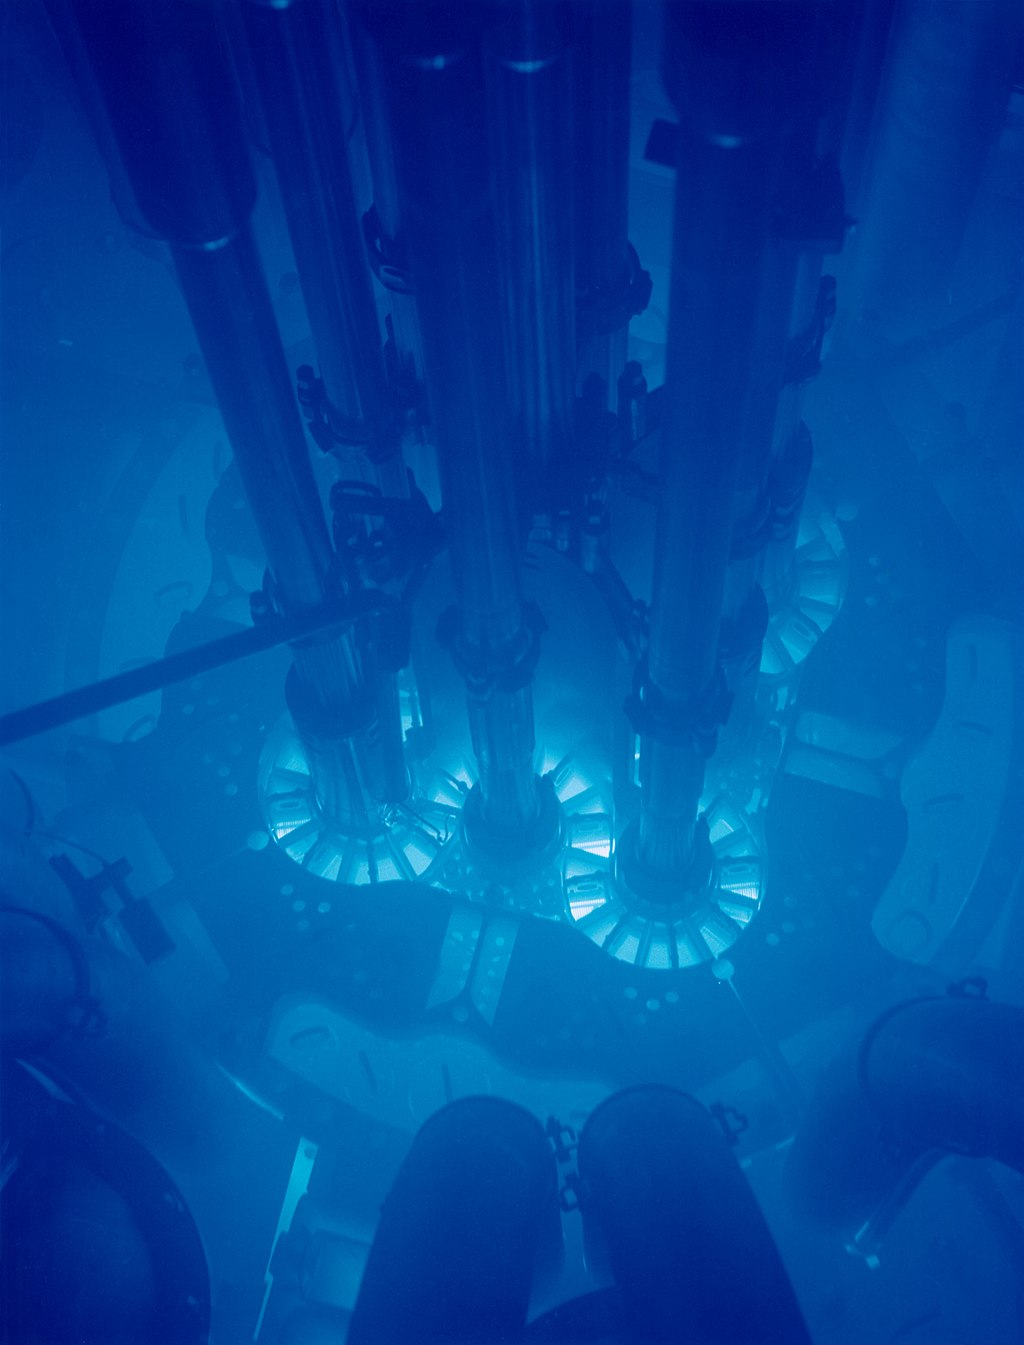
\includegraphics[height = 0.8\textwidth]{Cherenkov-reactor.jpg}}{\textcopyright Argonne National Laboratory\\Advanced Test Reactor core, Idaho National Laboratory}
	\caption{Cherenkov radiation in a nuclear reactor}
	\label{figure: Cherenkov reactor}
\end{minipage}
\hspace{0.05\textwidth}
\begin{minipage}{0.45\textwidth}
	\centering
	\copyrightbox[r]{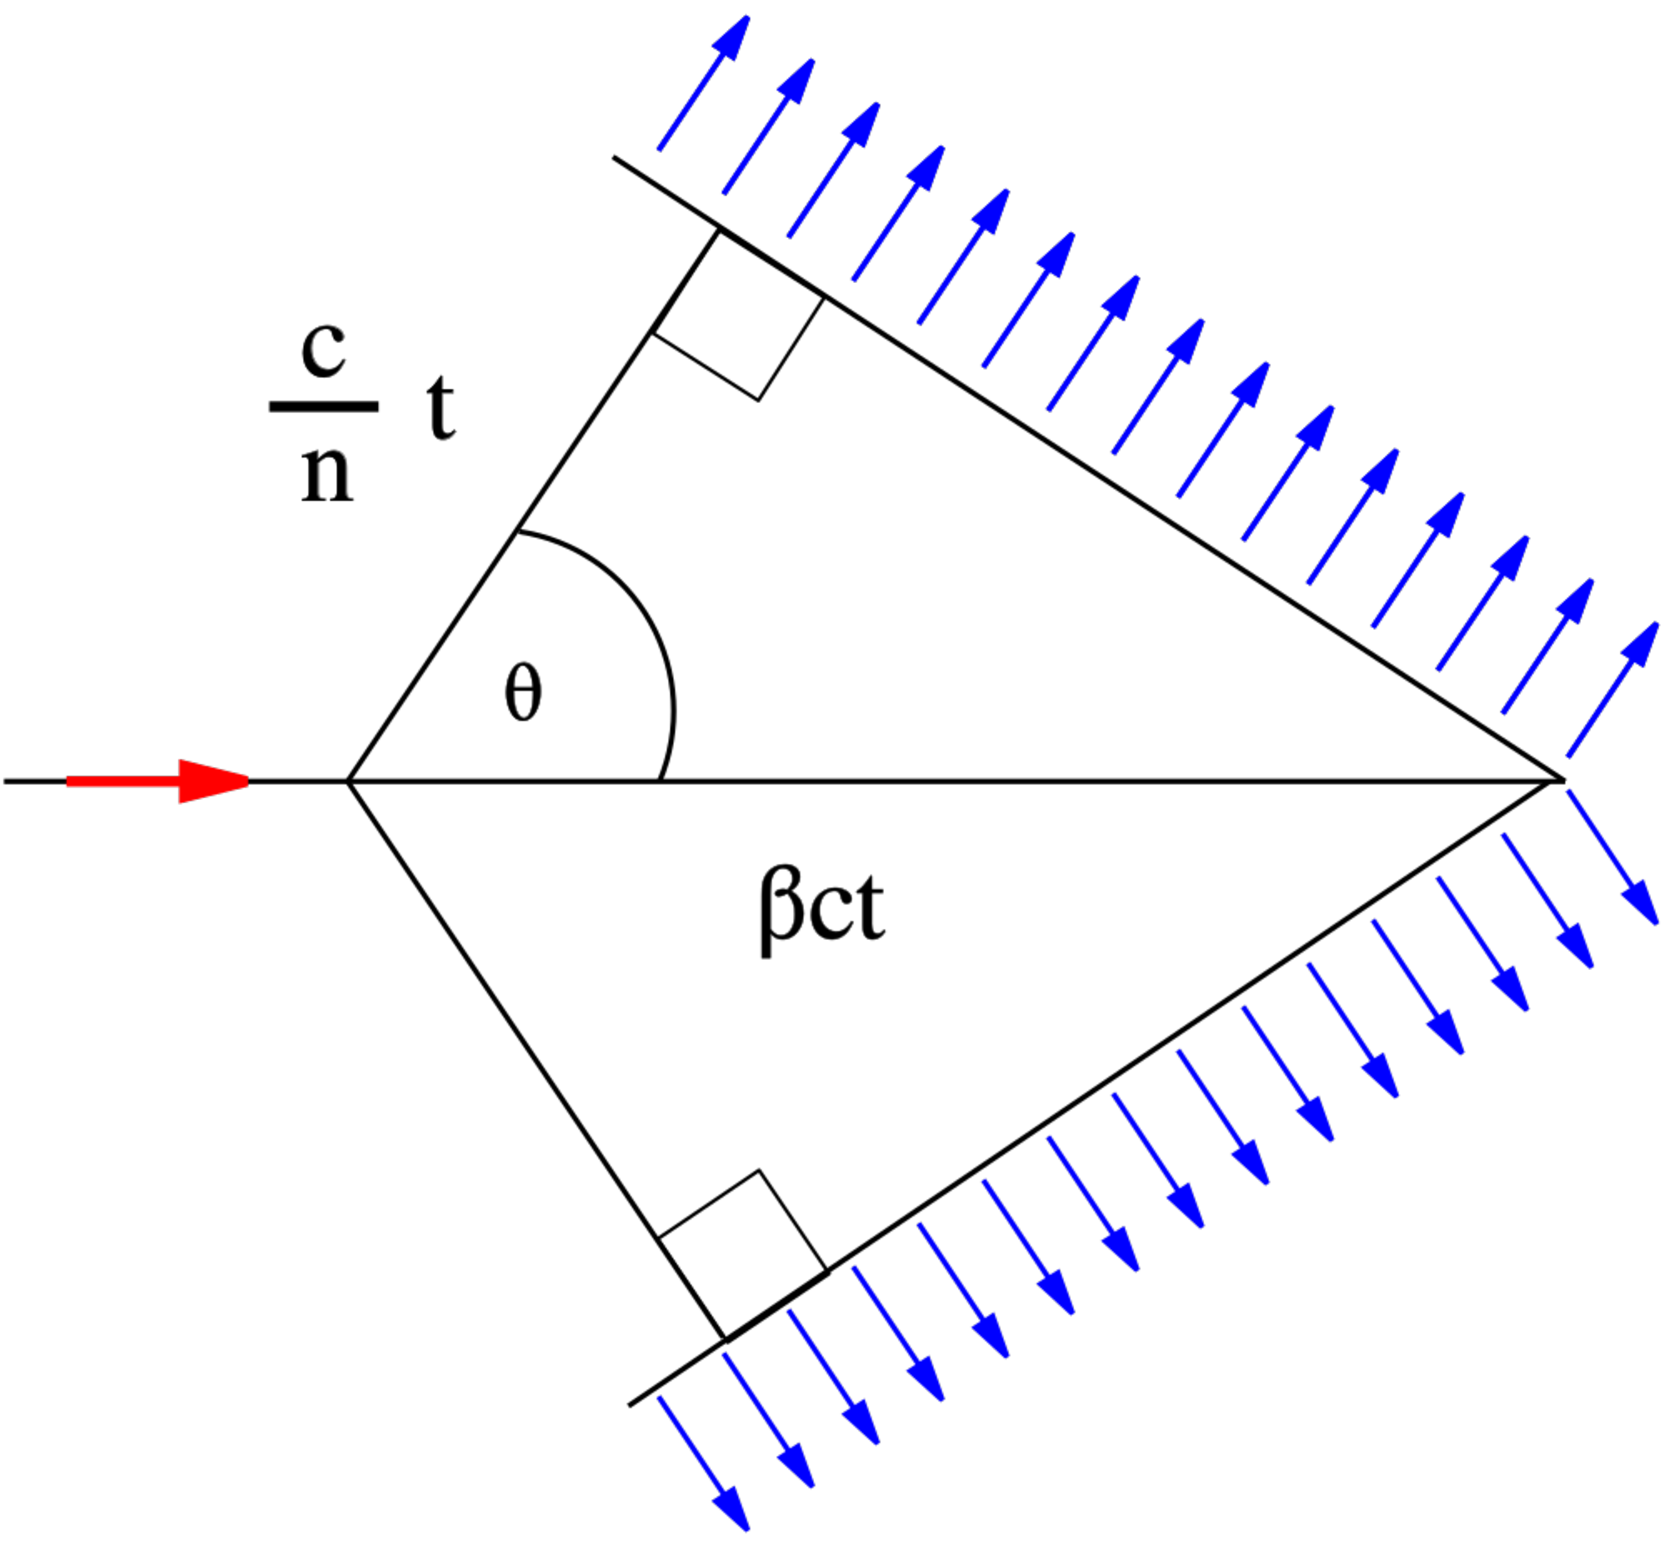
\includegraphics[height = 0.8\textwidth]{Cherenkov.pdf}}{\textcopyright Arpad Horvath}
	\caption{Diagrammatic representation of Cherenkov radiation}
	\label{figure: Cherenkov illustratie}
\end{minipage}
\end{figure}
Now if an observer is positioned at this Cherenkov angle all radio emission produced during the shower development reaches him/it at the same time, leading to constructive interference, hence the second condition is satisfied in ice for signals of $\approx 56°$
\section{Reconstruction}
It can pose a challenge to reconstruct the radio signals produced by the Cherenkov radiation as they are often obscured by background noise. A solution used in RadioReco is Information Field Theory (IFT) implemented in RadioReco by Welling et al.\cite{Welling_2021} which uses Bayesian inference to calculate the most likely radio signal, given recorded data.
\chapter{The Detector}
Both cosmic ray and neutrino detectors face the same main problem at the highest energies: the steeply falling flux requires large effective areas, wich leads to the construction of neutrino detectors with volumes on the cubic kilometer scale: IceCube. As we wish to detect neutrino's with even higher energies we turn to look at an array of detectors spanning multiple cubic kilometers: RNO-G.

One such detector is illustrated in figure \ref{fig:detector}.

The deep component of the detector can be split up in three parts: Two \textit{helper strings}, one \textit{power string} and the surface components. The helper strings are the 2 vertical cables shown on the right of the figure and each one houses 2 vertically polarized antennas (Vpols), one quadslot antenna for the horizontal polarization component (Hpol) and one radio pulser on each helper string which can be used to generate calibration signals.

The power string (the leftmost vertical cable) is more densely instrumented: At the bottom it houses a set of four Vpol and two Hpol antennas with a spacing of 1m and further up the string, with a spacing of 20m are three more Vpol antennas.

The signal from each of these antennae are fed into a low-noise amplifier directly above it, from there the signal is send to the data acquisition (DAQ) system at the surface via a Radio Frequency over Fiber (RFoF) cable. There it's again amplified, digitized and saved onto an SD card. This data is then transmitted via a Long Term Evolution (LTE) telecommunications network to a local server\footnote{There is additionally a Long Range Wide Area Network (LoRaWAN) antenna as backup in case of problems with the LTE network}, from where it is sent via a sattelite link.

There are solar panels as a power source who charge up battery banks, but as there is't enough light during the Greenland winters, there're plans to build wind turbines (with the problem being the possibly detectable RF noise the 'engine' produces)

\begin{figure}
	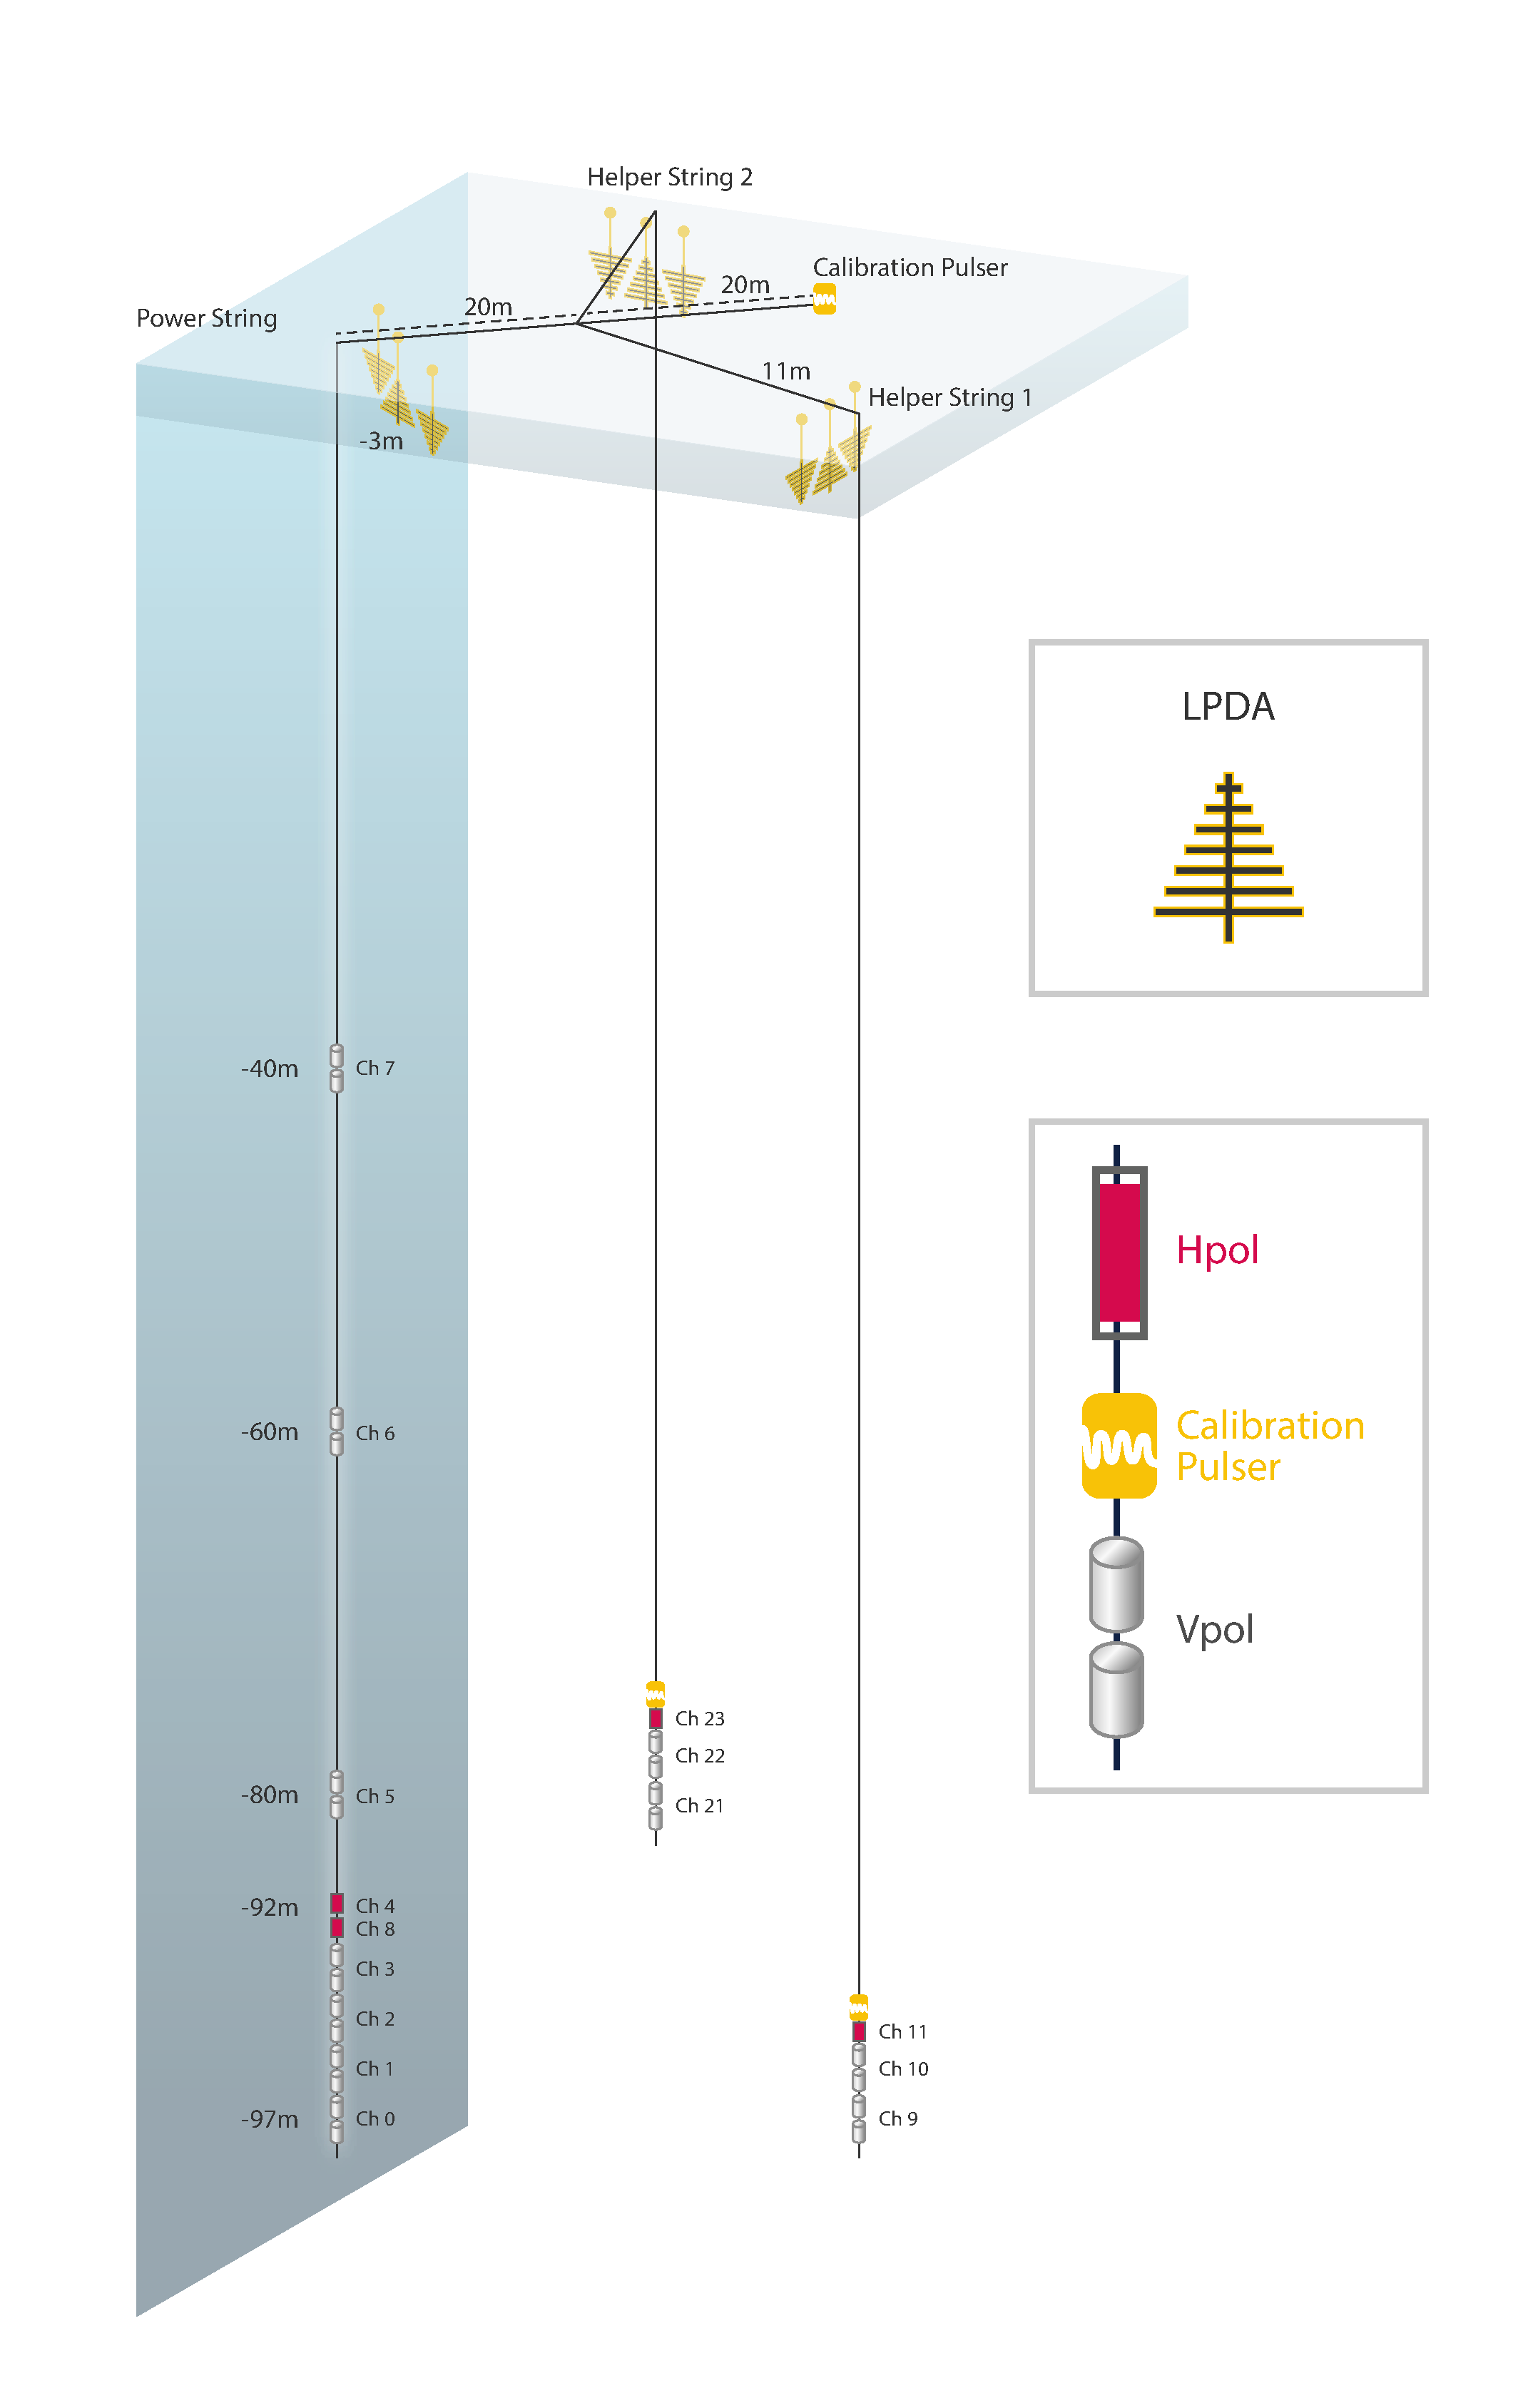
\includegraphics[width=0.9\textwidth]{figures/detector.pdf}	
	\caption{illustration of the detector}
	\label{fig:detector}
\end{figure}
\newpage
The radio signal from a neutrino often travels along both direct and refracted paths (designated DnR) to the deep array, this happens because the upper ice layer is a non-uniform medium where the signal trajectory is bent, as illustrated by a simulation in figure \ref{fig:path_illustration}. 

\begin{figure}[ht]
	\centering
	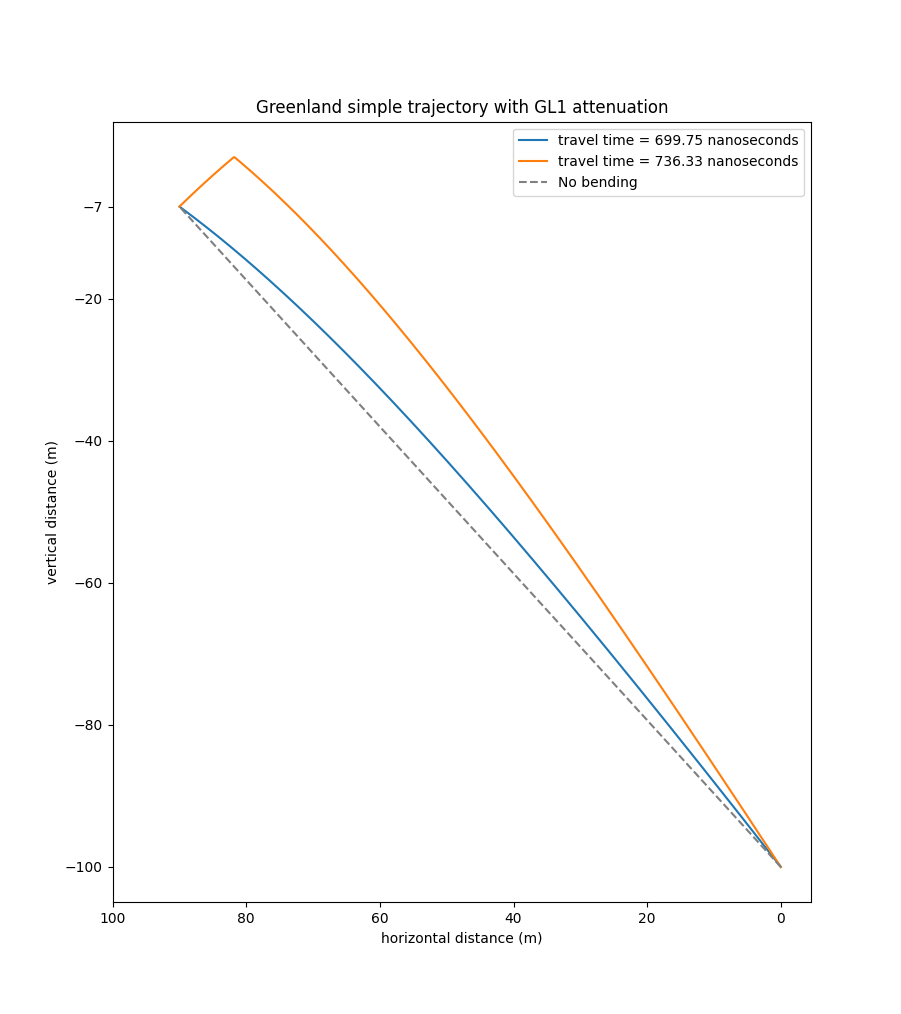
\includegraphics[width=0.6\textwidth]{figures/path_illustration.png}	
	\caption{illustration of a neutrino signal path}
	\label{fig:path_illustration}
\end{figure}


This double pulse characteristic would be a smoking-gun signature of an in-ice source. The two helper strings are needed for a full direction reconstruction. Three independent measurements are needed for azimuthal information, which is provided by the Vpol (Vertical polarization) antennas and placing the Hpol (Horizontal polarization) antennas at different depths on every string, both zentih and azimuth information will be provided for those signals. The helper strings' calibration pulsers, as well as one on the surface, will ensure regular monitoring of the performance of the station and provide information useful for precise calibration of the antenna geometry.

Christoph Welling did an investigation into energy reconstruction from the received signals\cite{Welling_2019} for air showers in one single station (as the RNO-G stations are so far apart this is the case here aswell) and he noticed that it is nescessary to know if the detector who observes an event falls inside or outside the Cherenkov cone to accurately reconstruct the primary particle energy as most over-estimated energies in his simulations are caused by events viewed from within the Cherenkov ring being mistaken for events outside of it. He went on to show that, if we somehow know if the shower was seen from inside or outside the ring from some extra source, that most outliers in the energy disappeared. It is shown by Hiller et al.\cite{Hiller_2017} that the combination of a muon detector with the radio detector might make the issue of confusion between being within or outside of the Cherenkov-ring disappear. Because of this the RNO-G stations are fitted with surface Log Periodic Dipole Antennas (LPDA), capable of detecting muons.
Note that this is for air showers, the radio signal from neutrinos show additional complexities.

\begin{figure}
	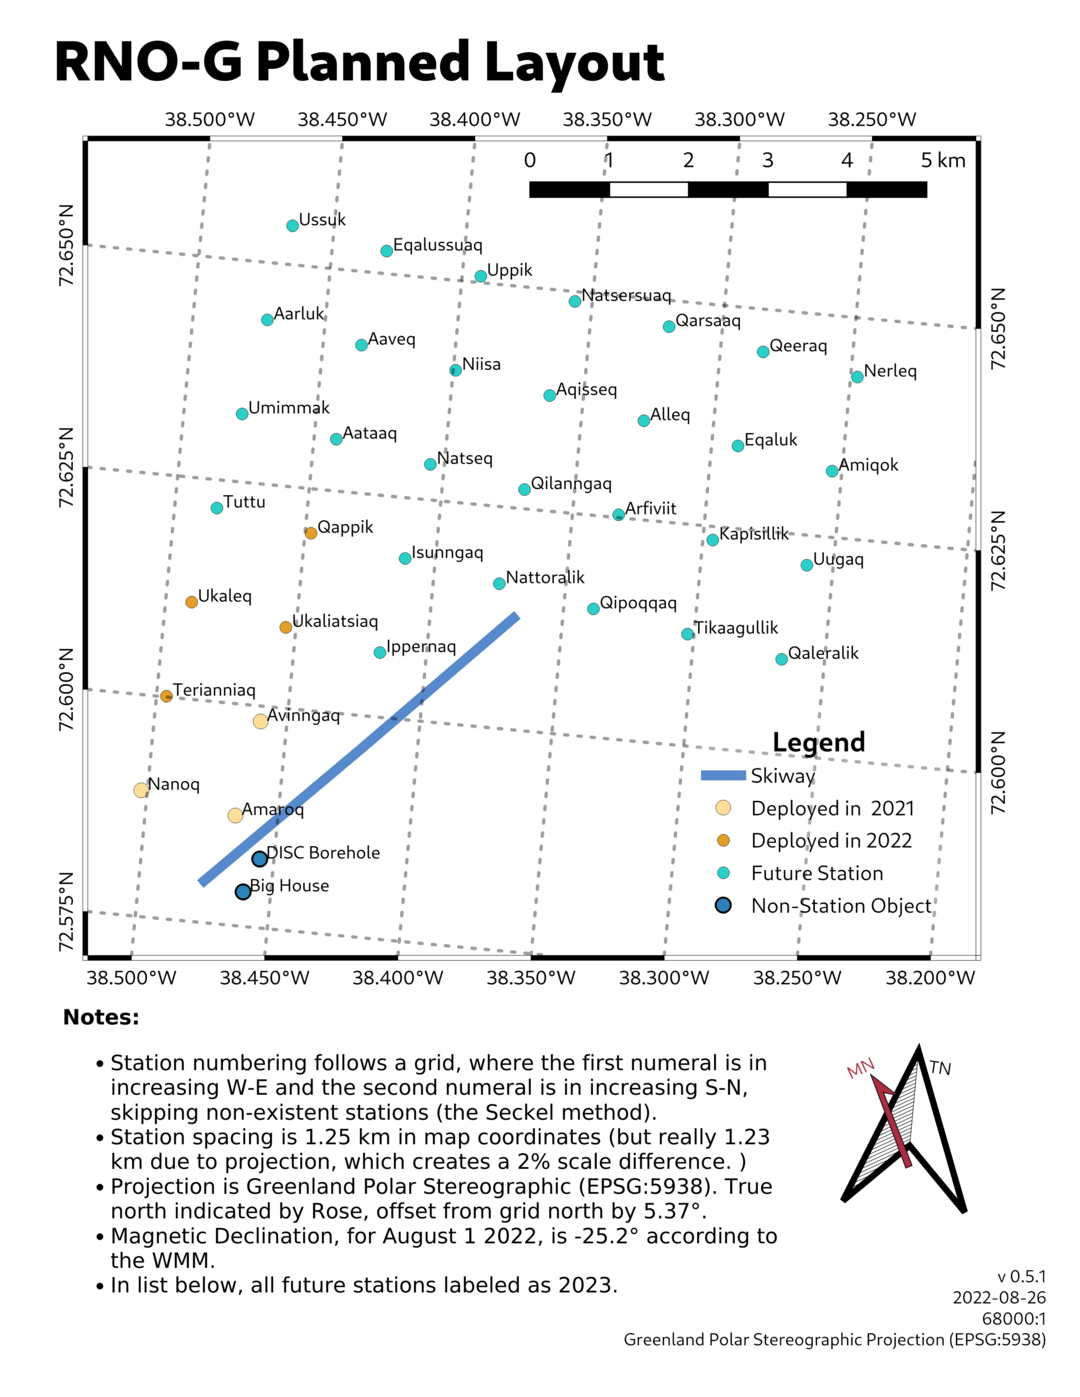
\includegraphics[width=\textwidth]{figures/station-map.png}	
	\caption{map of the station}
	\label{fig:station map}
\end{figure}

\chapter{Hybrid Ray tracer}
%----------------------------------------------------------------------------------------
%	ARTICLE CONTENTS
%----------------------------------------------------------------------------------------
\section{Introduction}
It has become apparent [citation needed] that complex ice models will be nescessary moving forward 
as the exponential ice model fails to fit the density curve. 
The ideal software for radio wave propagation through
ice is radiopropa\cite{Winchen_2019}, but due to the way it works you'll have
to know the start point , the end point and the launch angle of your ray to
work out the path. With the exponential model the launch angle is known from solving a simple 
equation.
However for a more difficult ice model the launch angle can't be know a priori.
Work has been done on this by B. Oeyen et al. \cite{2022icrc.confE1027O}, 
where they created a ray tracer which iteratively finds the solution, 
called the "iterative ray tracer".
The full explanation of how their algorithm works can be found in the mentioned paper. 
This is however a sub-optimal solution in python as an optimalisation library 
will generally work faster, work
had been done on trying to implement such an algorithm but this attempt failed.
As I saw this work I had an idea to combine the iterative ray tracer and the code using the 
optimisation libraries (a so called "minimizer"), to come up with the algorithm that will 
be discussed in this chapter: The hybrid ray tracer, in the source code called the "hybrid
minimizer".

It succeeds in more rapidly tracing the path from the event
to the detector, is more accurate and also arrives closer to the detector as the final result is
not limited by the final drawn sphere size but by a given tolerence.

\section{How it works}
\begin{figure}[h!]
	\centering
	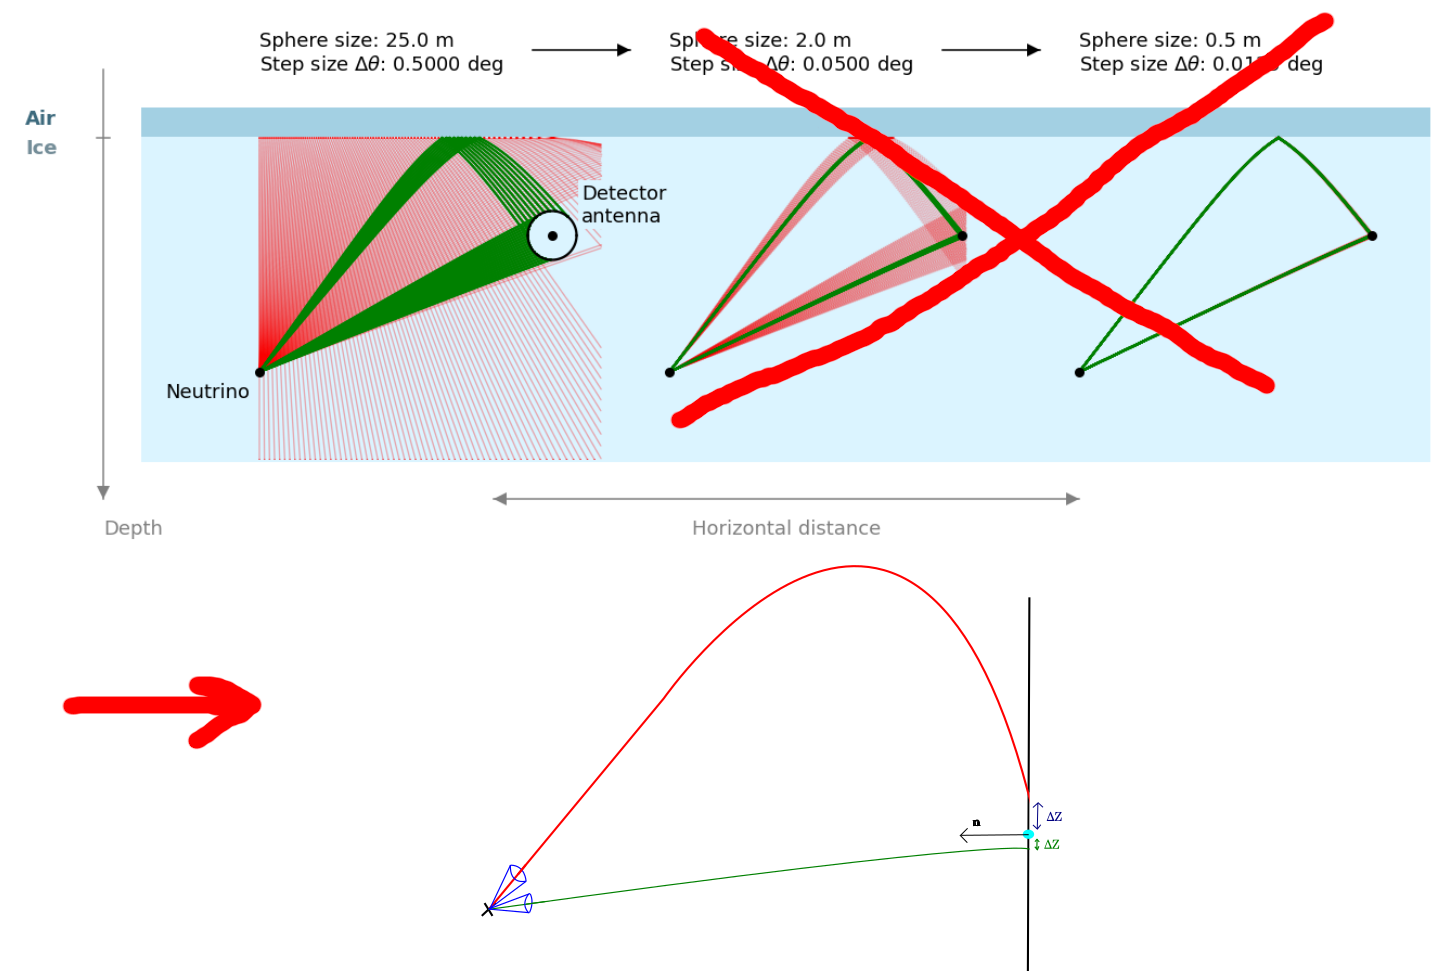
\includegraphics[width=\textwidth]{figures/explanation.png}
	\caption{explanation of the hybrid method}
	\label{fig:explanation}
\end{figure}
The hybrid minimizer can be seen as an extension of the iterative raytracer, it
checks after the first loop (as explained in the paper by B. Oeyen et al.
\cite{2022icrc.confE1027O}) if there are 2 distinct launch regions, if this is
the case it breaks out of the loop 
as is visually explained using a modified version of B. Oeyen et al. their figure in the top
part of figure \ref{fig:explanation}. 
It then goes on to use the scipy.optimize.minimize module
to find the solutions in the respective angle intervals
as shown in the bottom part of figure \ref{fig:explanation} (minimizing $\Delta z$). If it doesn't find 2
distinct regions after the first loop, it falls back on the iterative ray tracer. 
\section{random number generator}
To test the hybrid minimizer the numpy random module was used to generate
random coördinates, the considered square (as there is only a z component to the
ice model the 3D problem is essentially only a 2D problem) is x:0.1km,4km and
z:-0.1km,-3km.\footnote{This start at 100m depth was to get around issues concerning events that 
won't even trigger in a full simulation}
\section{Performance Optimalisation}
\subsection{Length of the normal vector}
\begin{figure}[h!]
	\centering
	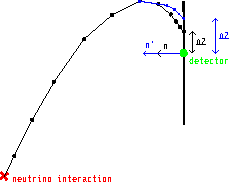
\includegraphics[width=0.7\textwidth]{figures/PrincipleNormIllu.pdf}
	\caption{how normal vector size influences the stepsize}
	\label{fig:normexpl}
\end{figure}
As visually explained in figure \ref{fig:normexpl}, the size of the normal vector seems to
influence how big the ray tracer's step size is taken close to the detector. This
thus influences the convergence and time taken. The results of varying this are shown
in figures \ref{fig:norminfl} and \ref{fig:norminfl2}.
Looking at these figures the first optimization conclusion is as expected: 
take the normal vector length to be 1 meter.
\subsection{ztol}
We'll now change the tolerence on the vertical distance away from the detector which is deemed
accepted i.e in figure \ref{fig:normexpl} if $\Delta z$ is below this threshold it's accepted.
The results are shown in figures \ref{fig:ztolinfl} and \ref{fig:ztolinfl2}.
From which we can conclude the second optimization conclusion: take ztol to be 0.05 m.
\subsection{Sphere Size \& Step Size}
As explained in Oeyen et al.'s work, the initial rays are sent out in steps of a
certain angle and with a sphere around the detector (as can also be seen at the top of
figure \ref{fig:explanation}, but for clarification I again refer to their
paper). The sphere size and step size weren't jet optimized. But as
this is the slowest step in the hybrid ray tracer this was optimized here (only
the initial sphere and step size as those are relevant for the hybrid
raytracer) as seen in figures \ref{fig:SphereStepInfl} and \ref{fig:SphereStepFinal}.

\begin{figure*}
	\centering
\begin{minipage}{0.49\textwidth}
	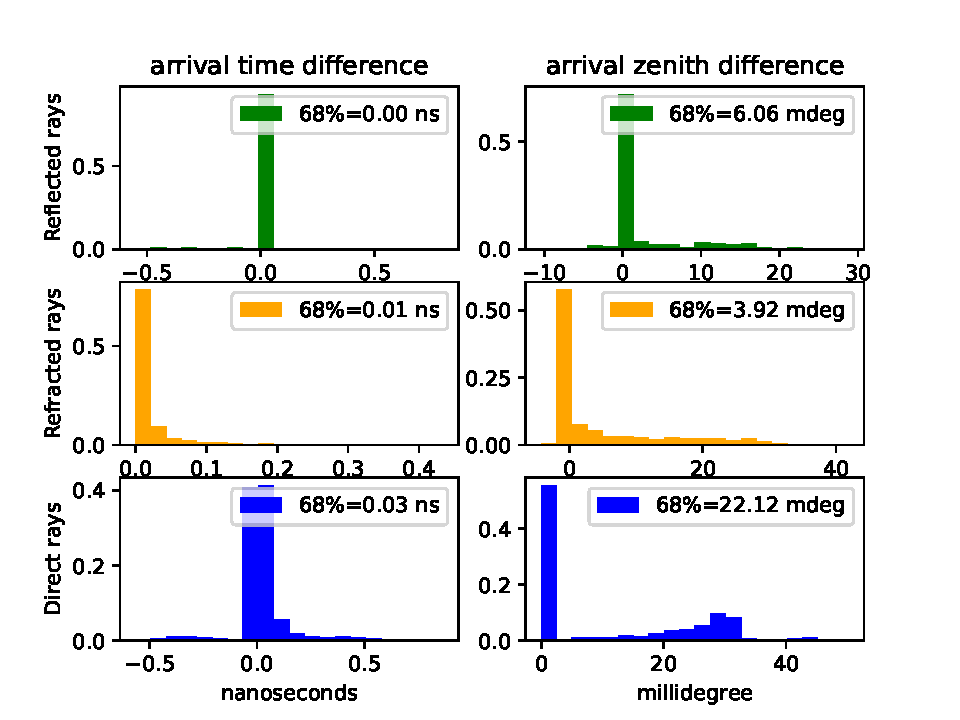
\includegraphics[width=1.1\textwidth]{figures/hybrid_comparison_N_1000.pdf}
	\caption{Hybrid}
	\label{fig:acchyb}
\end{minipage}
\begin{minipage}{0.49\textwidth}
	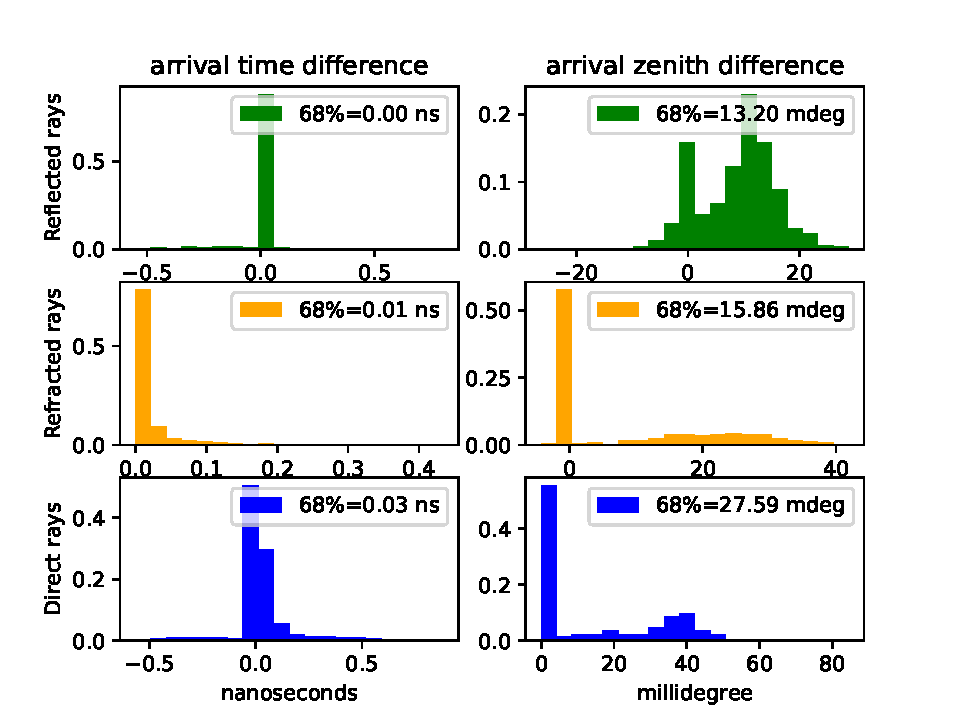
\includegraphics[width=1.1\textwidth]{figures/iterative_comparison_N_1000.pdf}
	\caption{Iterative}
	\label{fig:accit}
\end{minipage}
\end{figure*}

\begin{figure}
	\centering
	\begin{minipage}{\textwidth}
		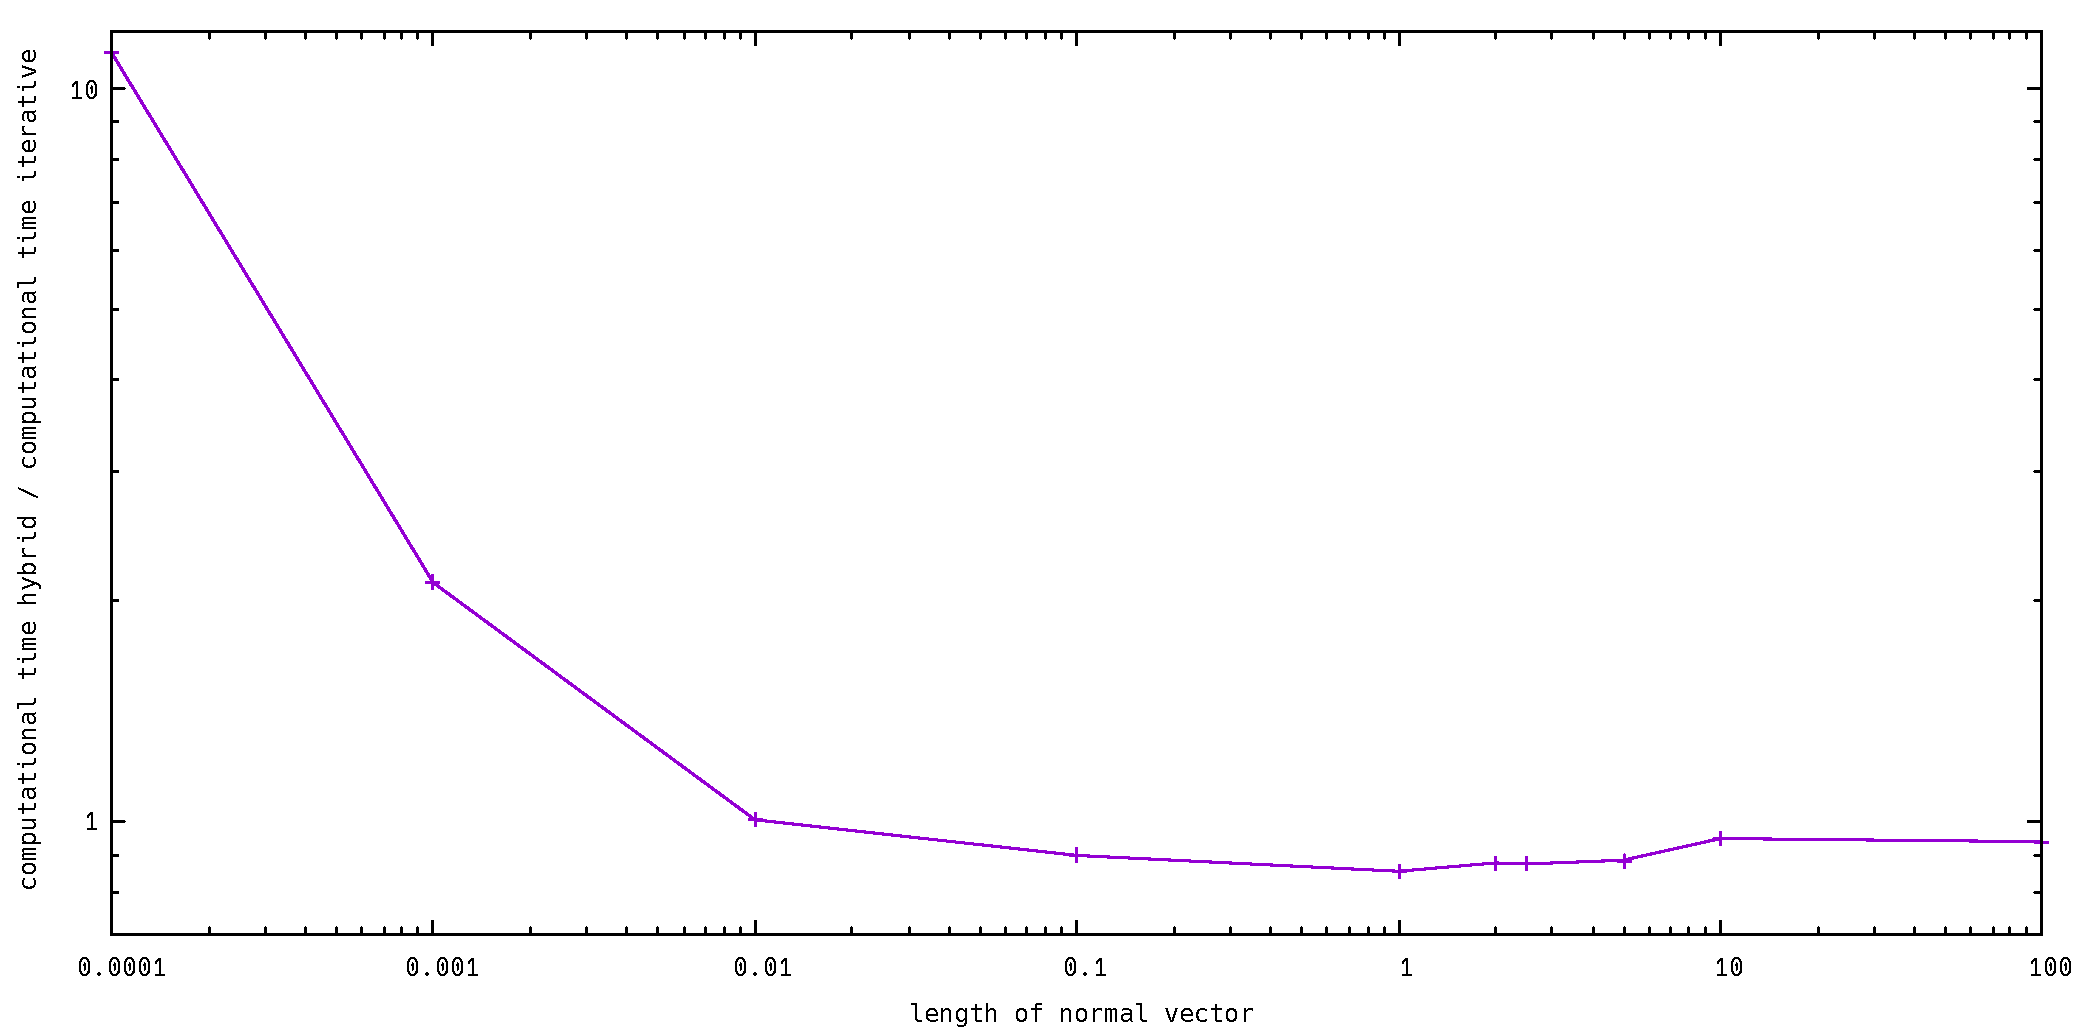
\includegraphics[width=0.8\textwidth]{figures/NormVsTime.pdf}
	\end{minipage}
	\begin{minipage}{\textwidth}
		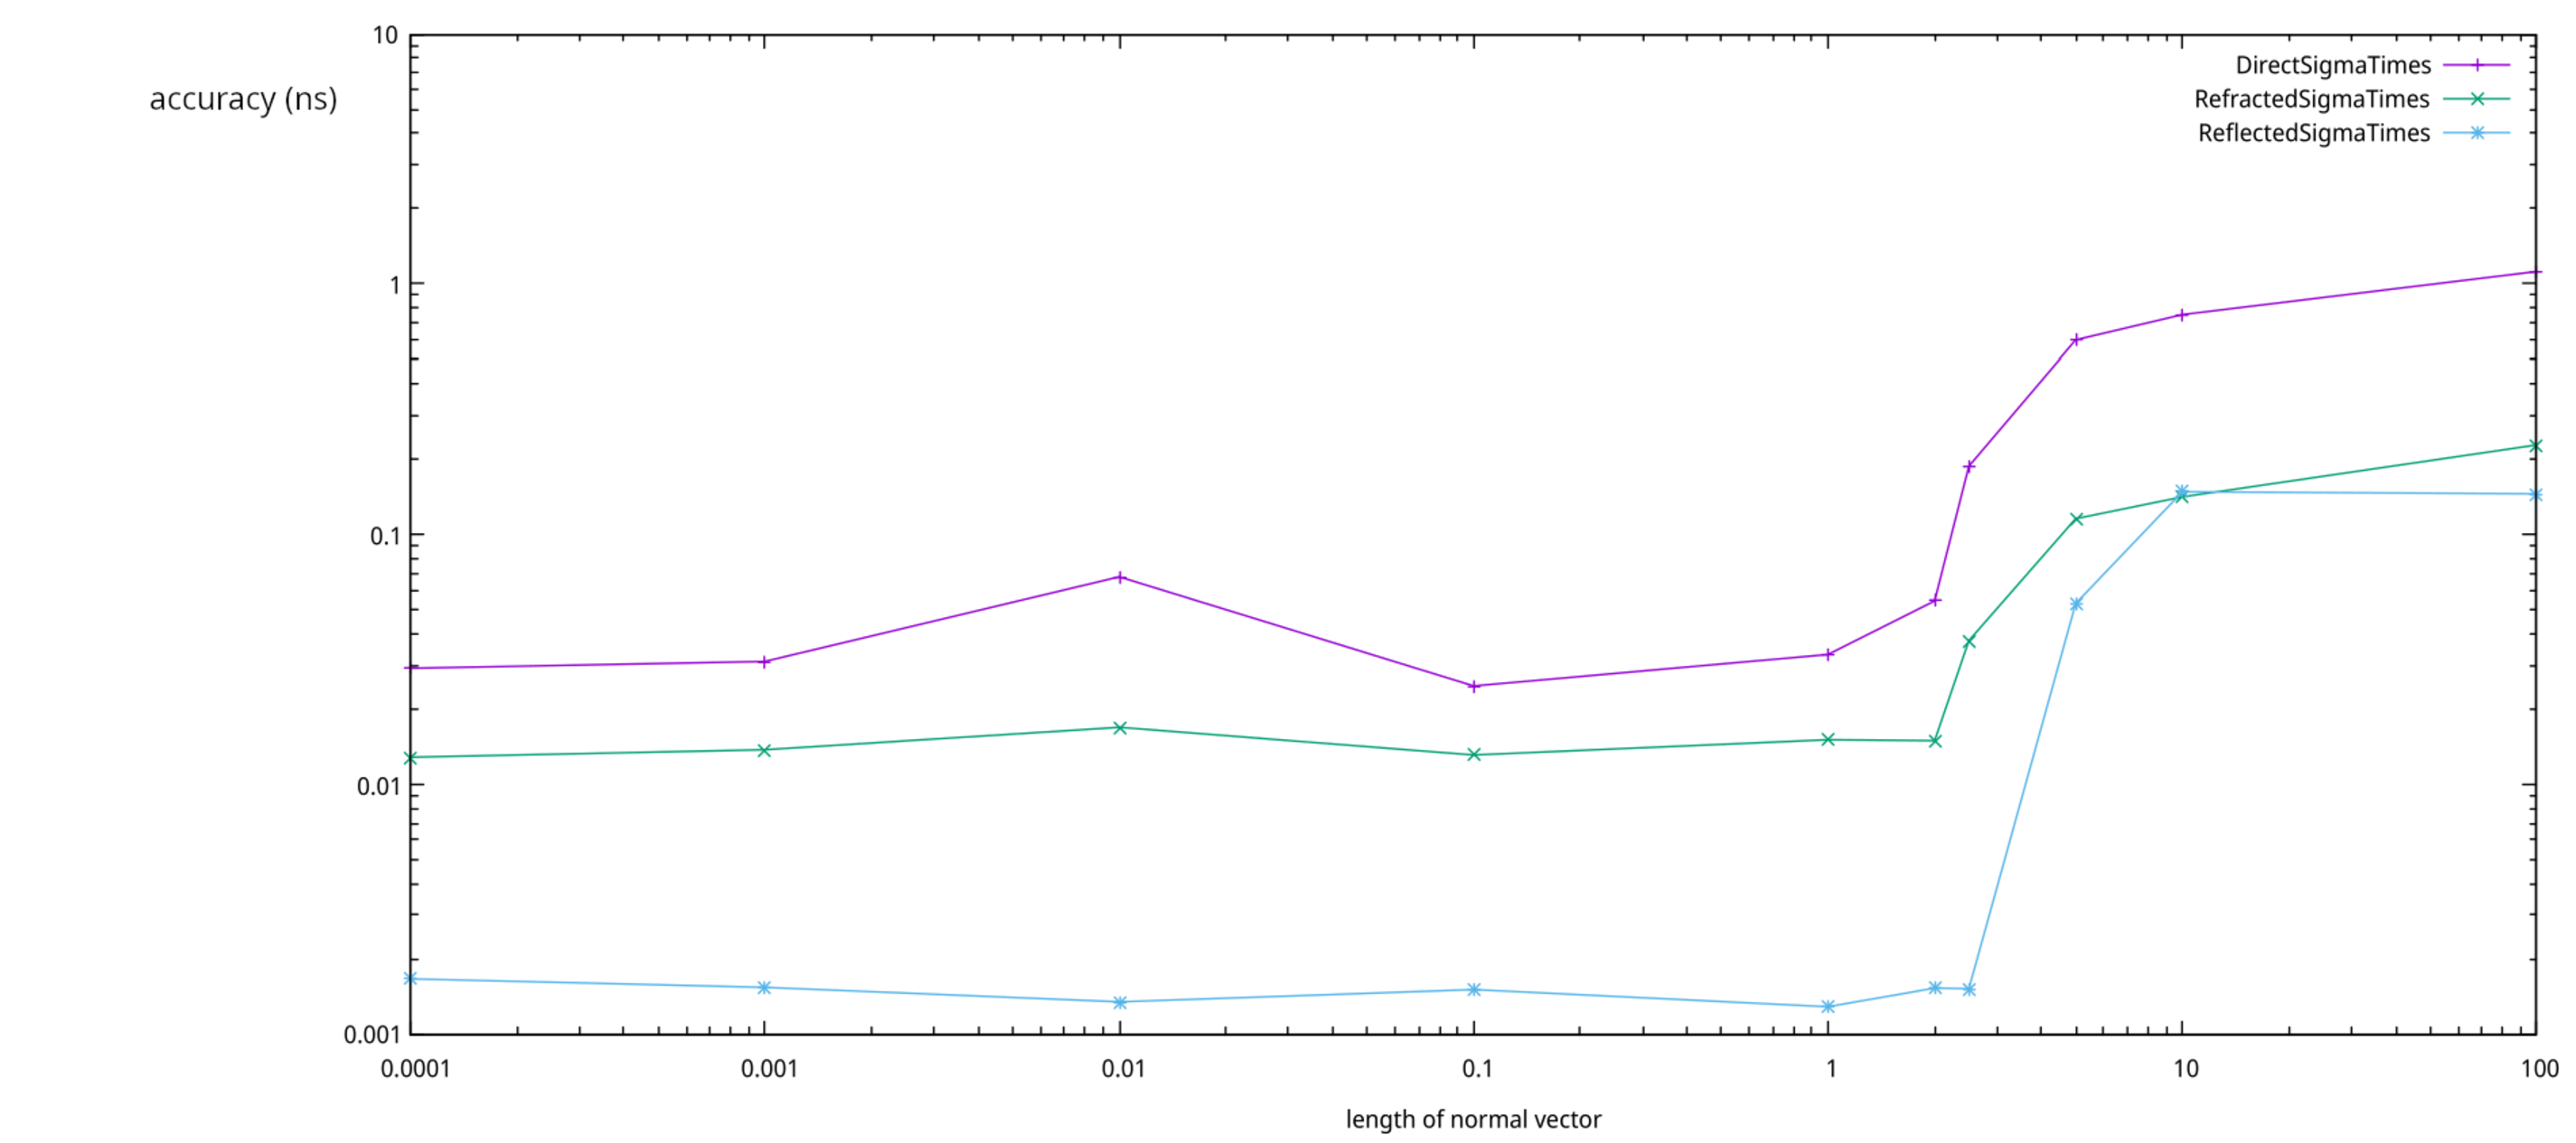
\includegraphics[width=0.8\textwidth]{figures/NormVsSigmaTime.pdf}
	\end{minipage}
\caption{influence of the length of the normal vector}
\label{fig:norminfl}
\end{figure}
\begin{figure}
	\centering
	\begin{minipage}{\textwidth}
		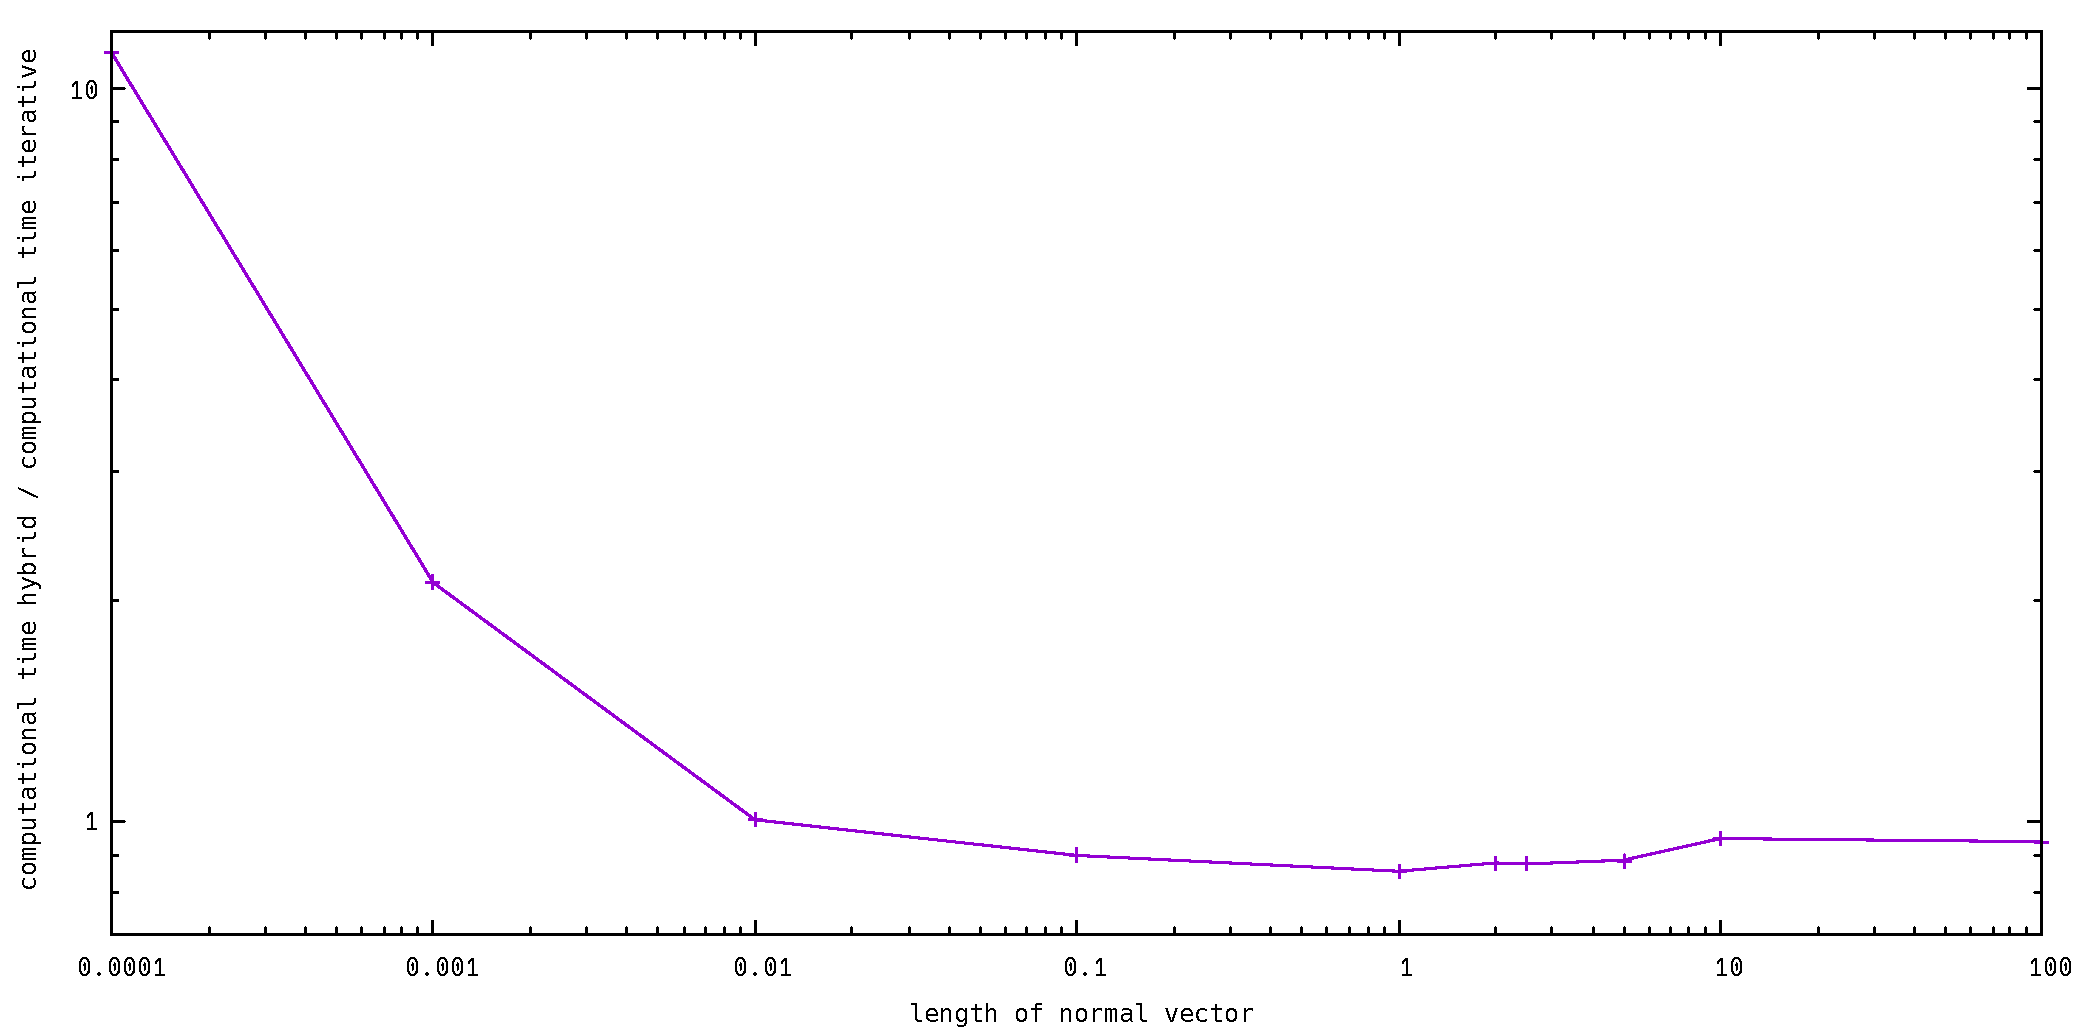
\includegraphics[width=0.8\textwidth]{figures/NormVsTime.pdf}
	\end{minipage}
	\begin{minipage}{\textwidth}
		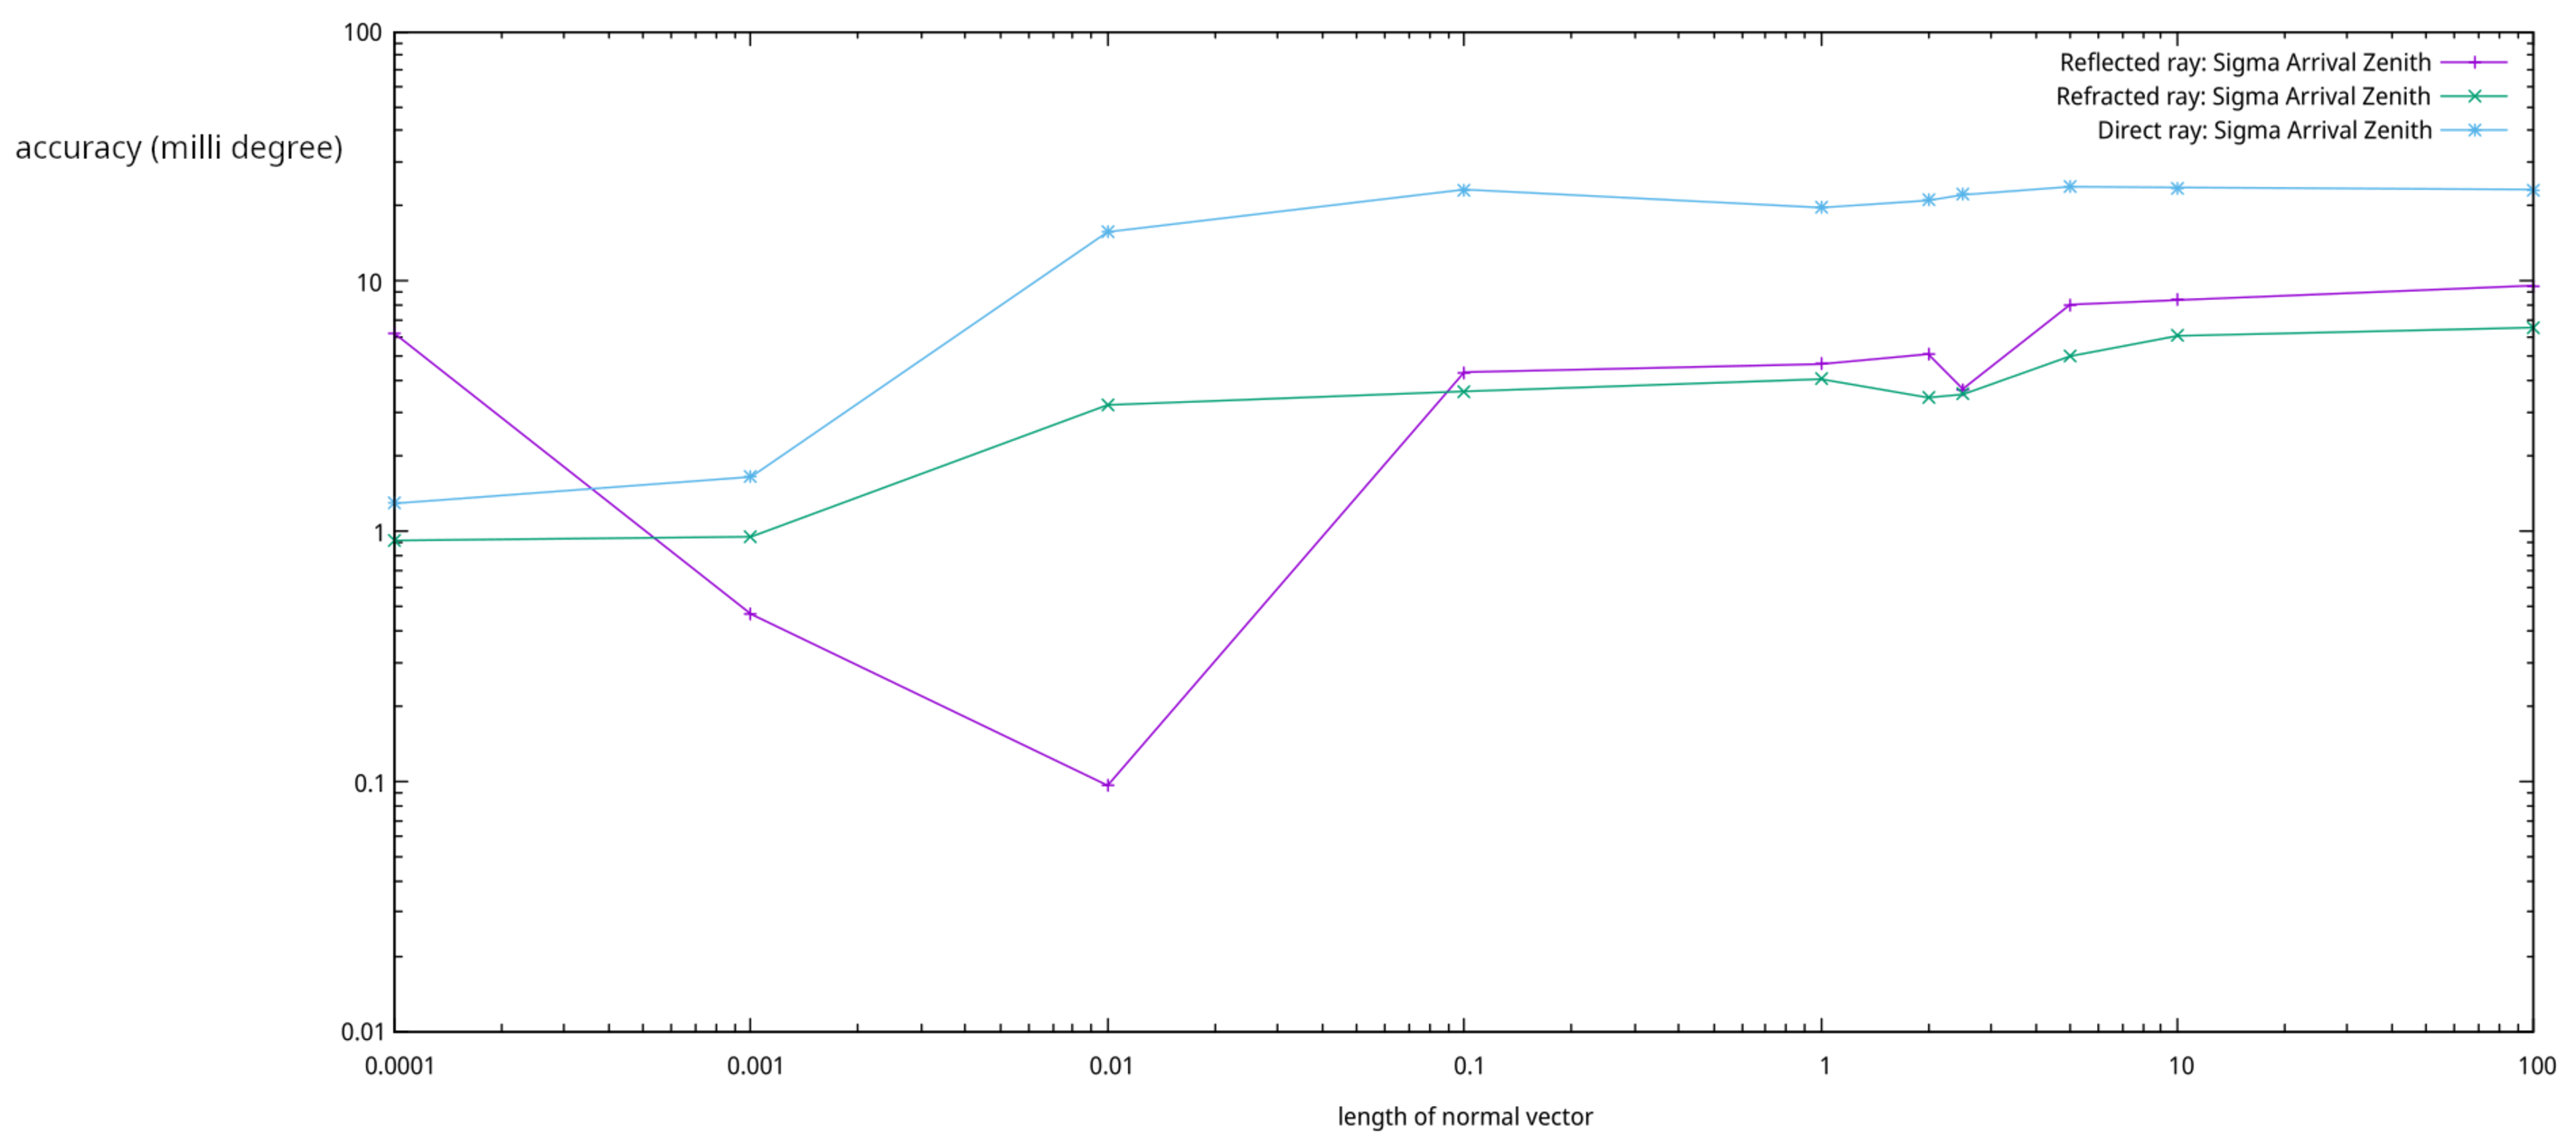
\includegraphics[width=0.8\textwidth]{figures/NormVsSigmaAZ.pdf}
	\end{minipage}
\caption{influence of the length of the normal vector}
\label{fig:norminfl2}
\end{figure}

\begin{figure}
	\centering
	\begin{minipage}{\textwidth}
		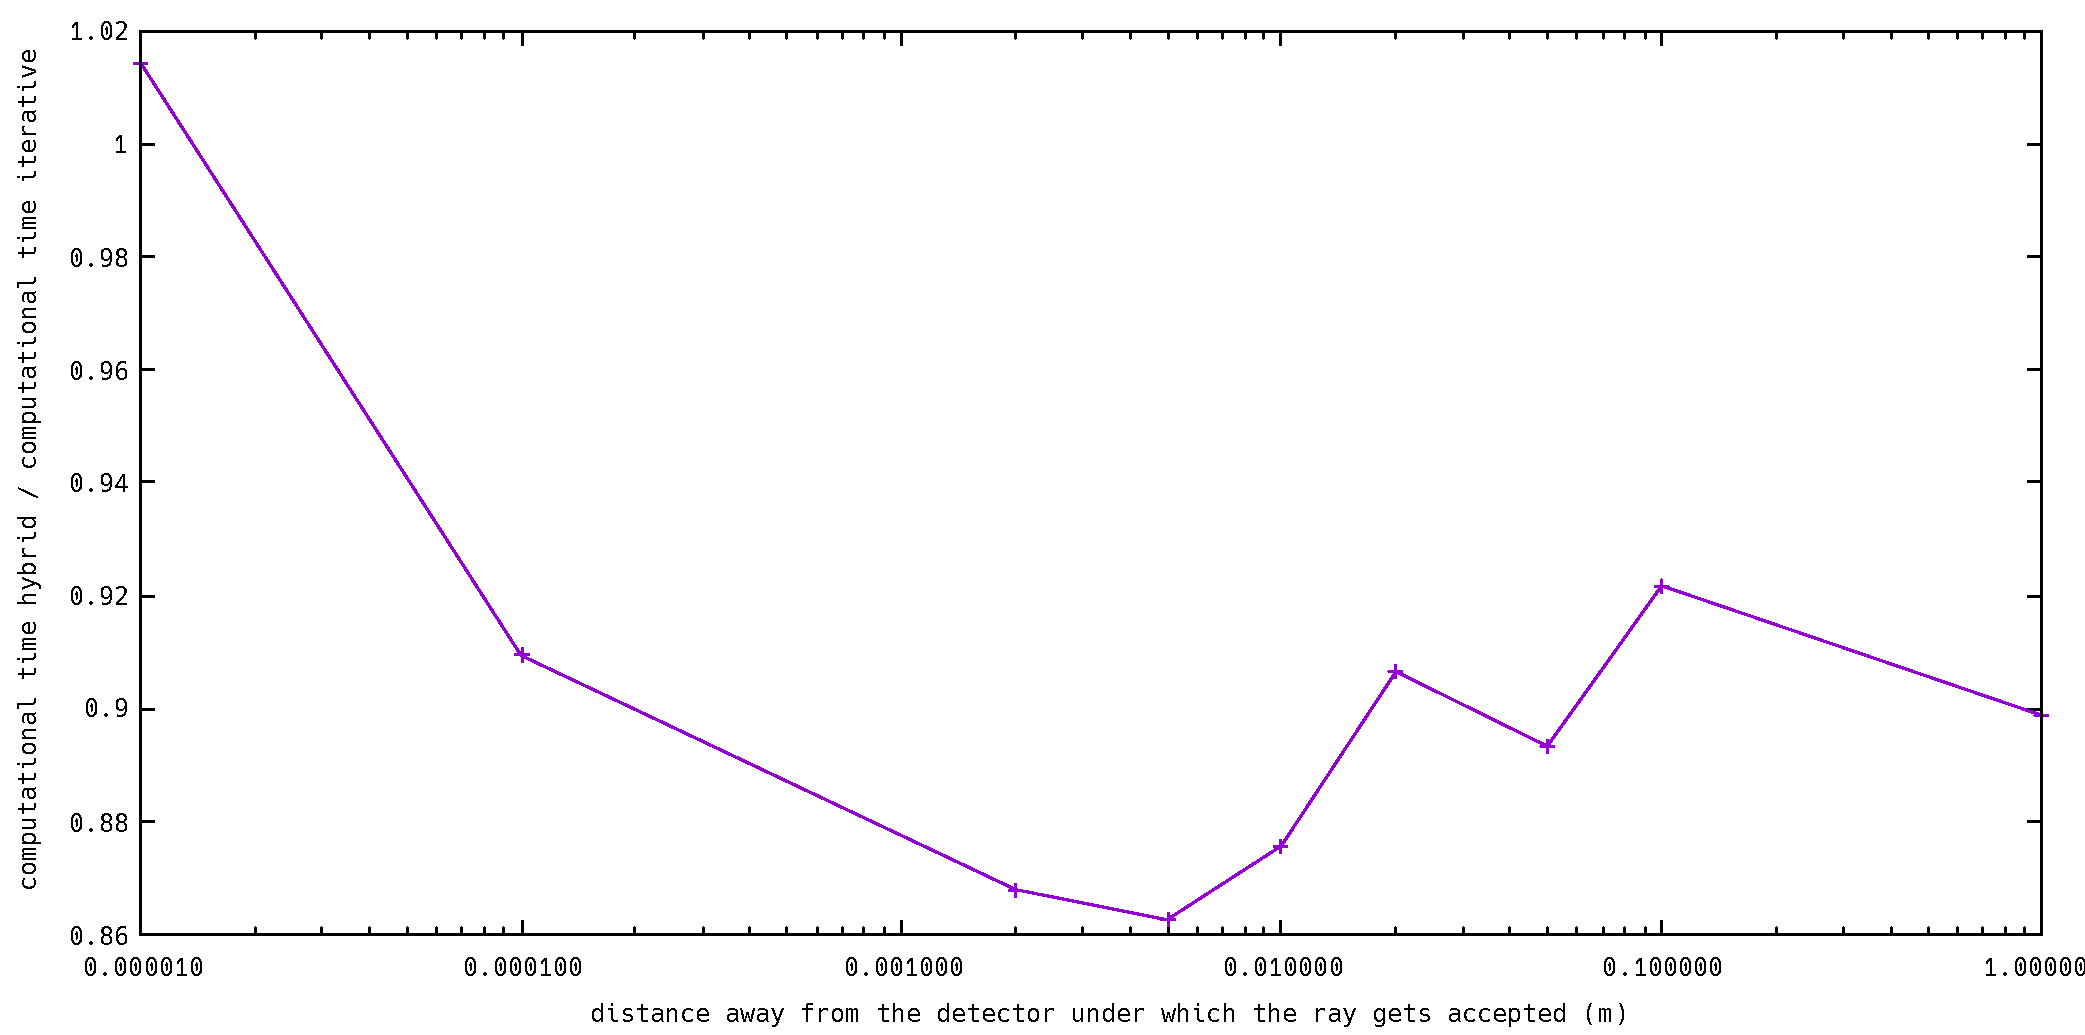
\includegraphics[width=0.8\textwidth]{figures/ZtolVsTime2.pdf}
	\end{minipage}
	\begin{minipage}{\textwidth}
		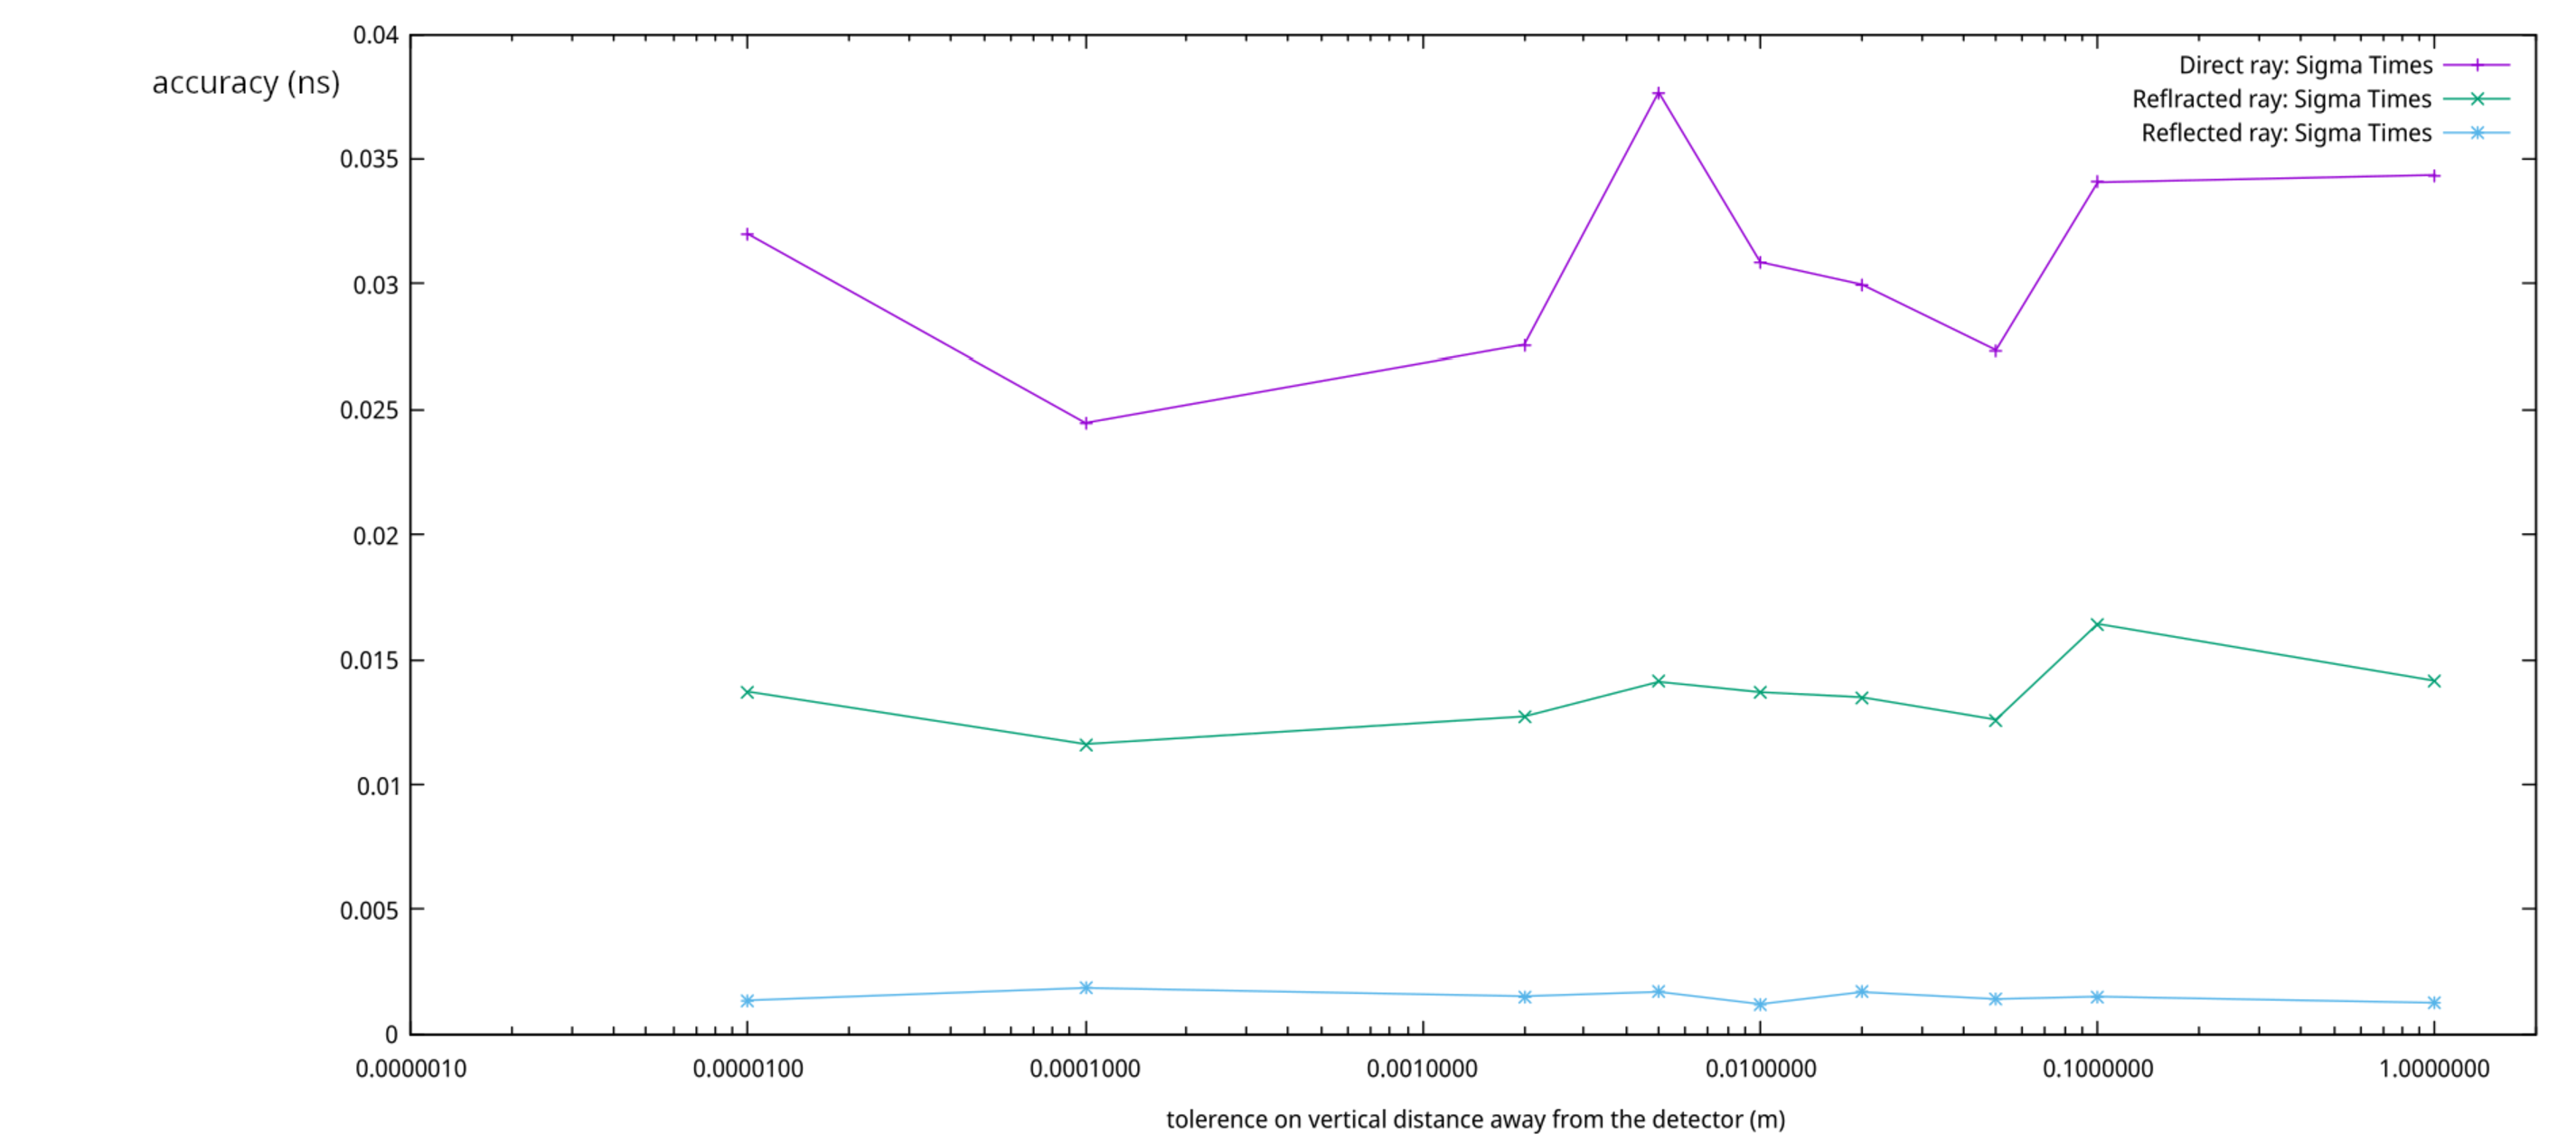
\includegraphics[width=0.8\textwidth]{figures/ZtolVsSigmaTime.pdf}
	\end{minipage}
\caption{influence of the tolerence on vertical distance}
\label{fig:ztolinfl}
\end{figure}

\begin{figure}
	\centering
	\begin{minipage}{\textwidth}
		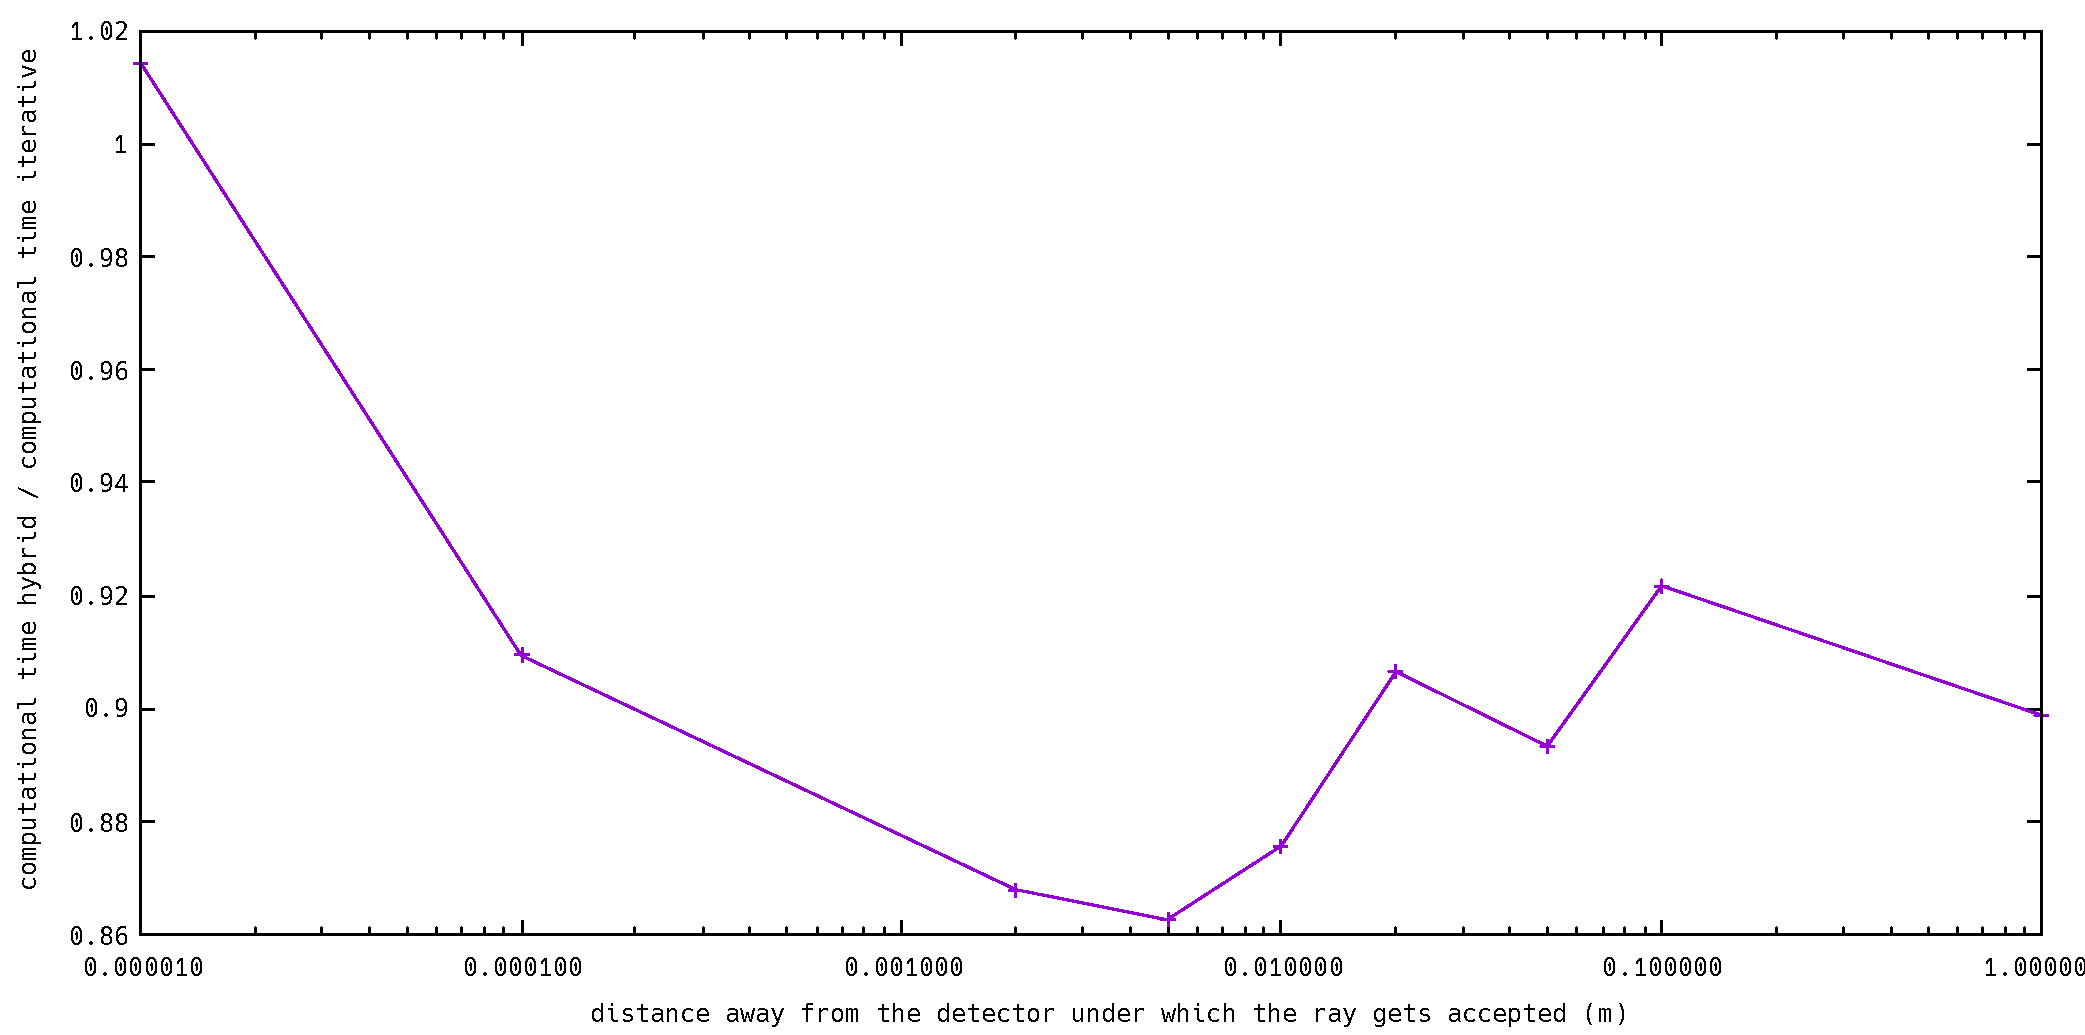
\includegraphics[width=0.8\textwidth]{figures/ZtolVsTime2.pdf}
	\end{minipage}
	\begin{minipage}{\textwidth}
		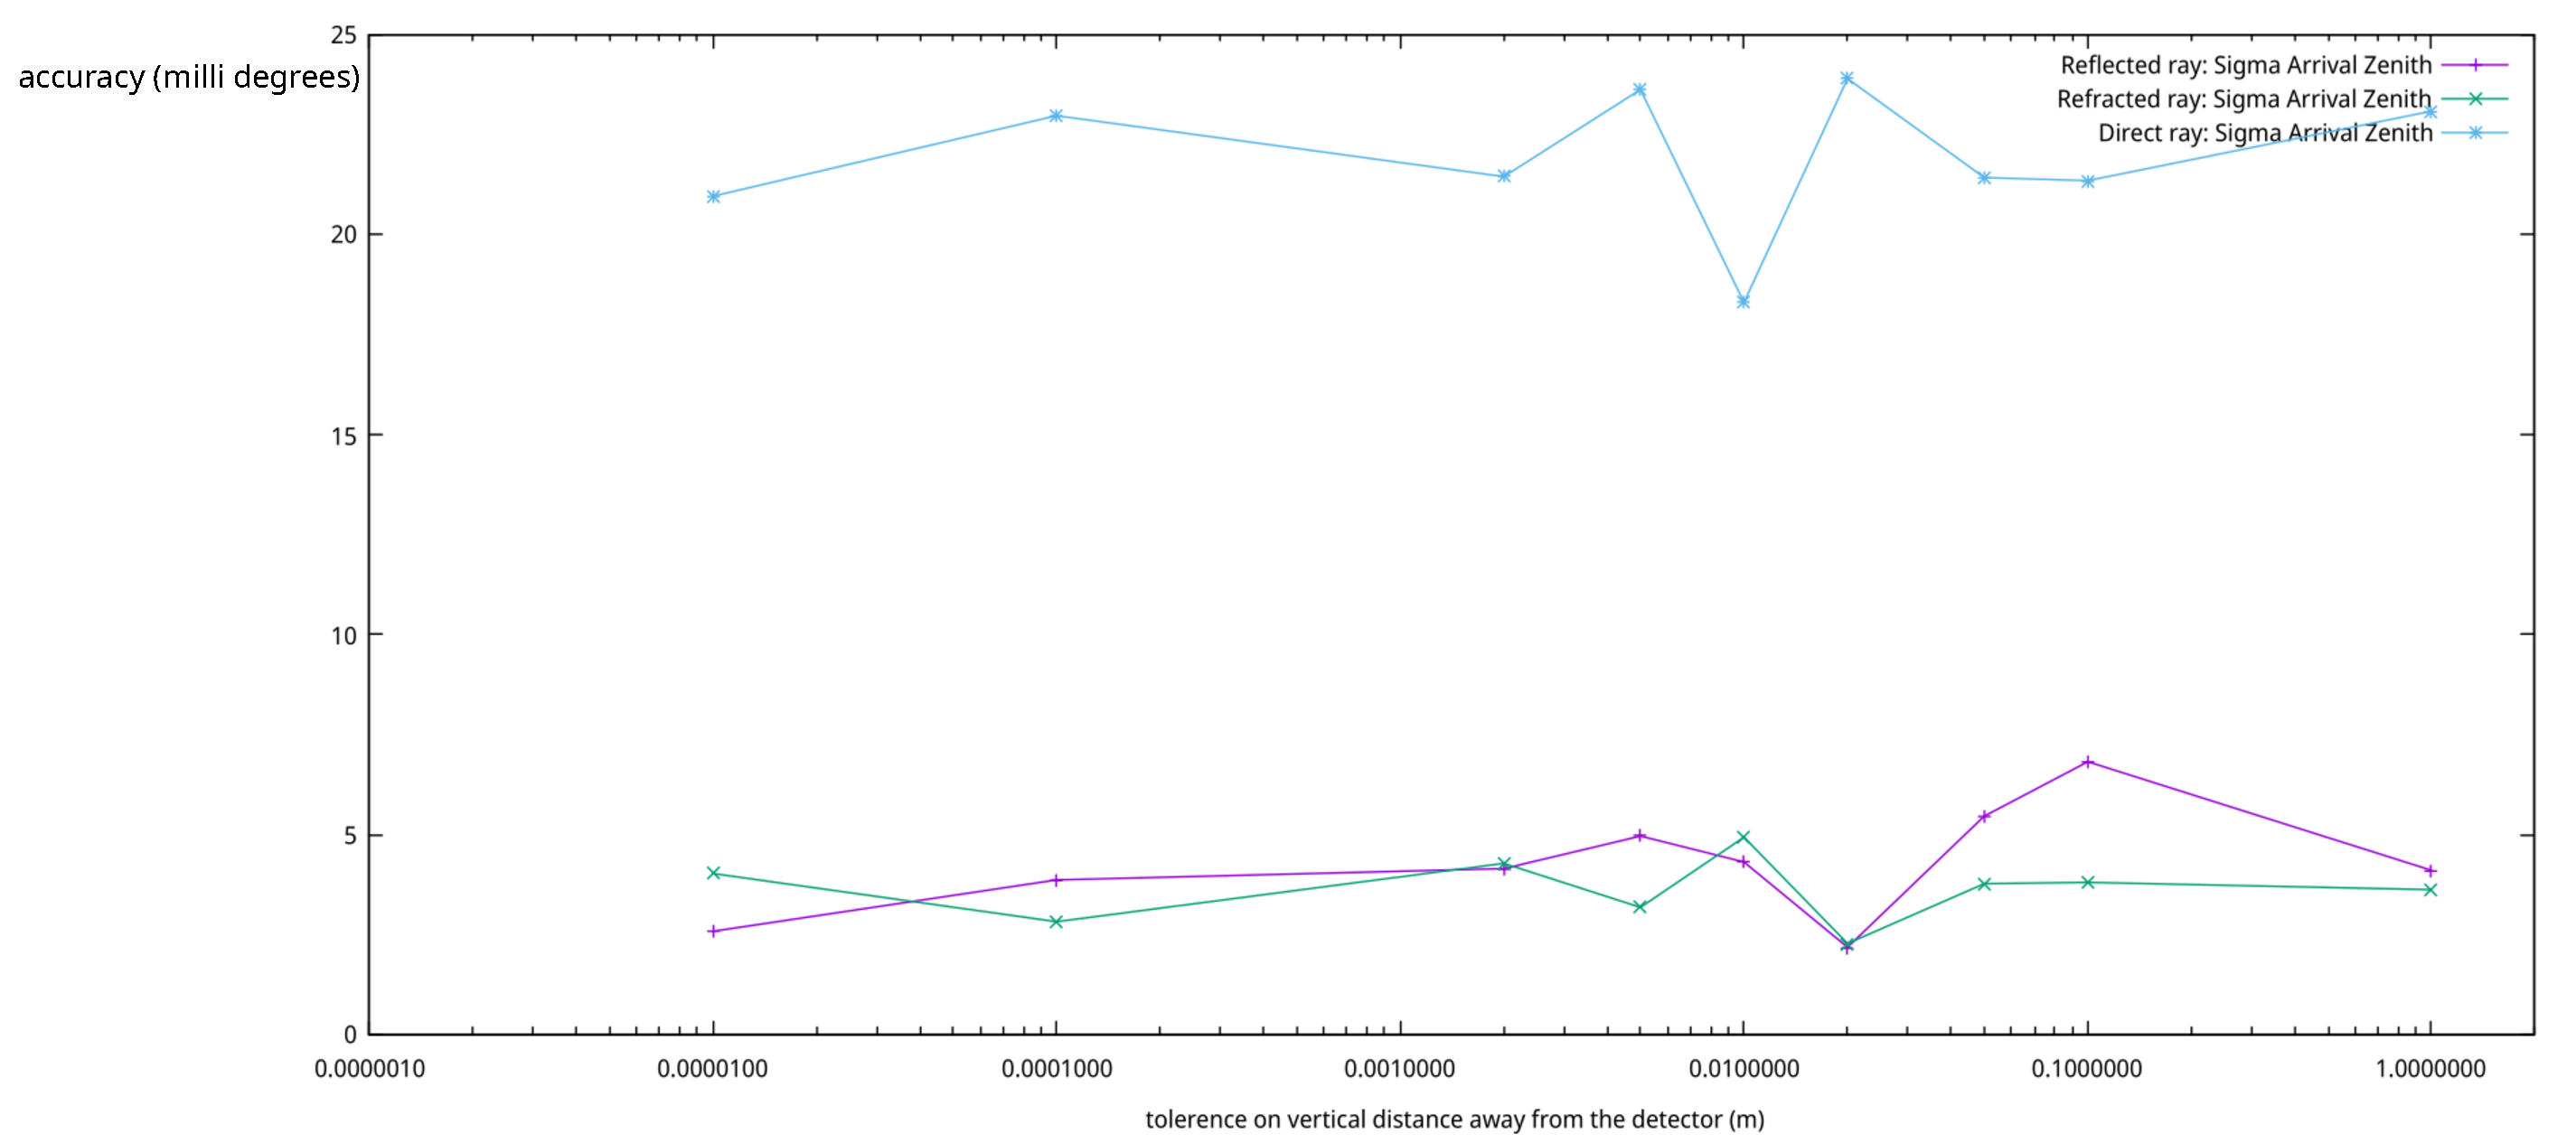
\includegraphics[width=0.8\textwidth]{figures/ZtolVsSigmaAZ.pdf}
	\end{minipage}
\caption{influence of the tolerence on vertical distance}
\label{fig:ztolinfl2}
\end{figure}

\begin{figure}
	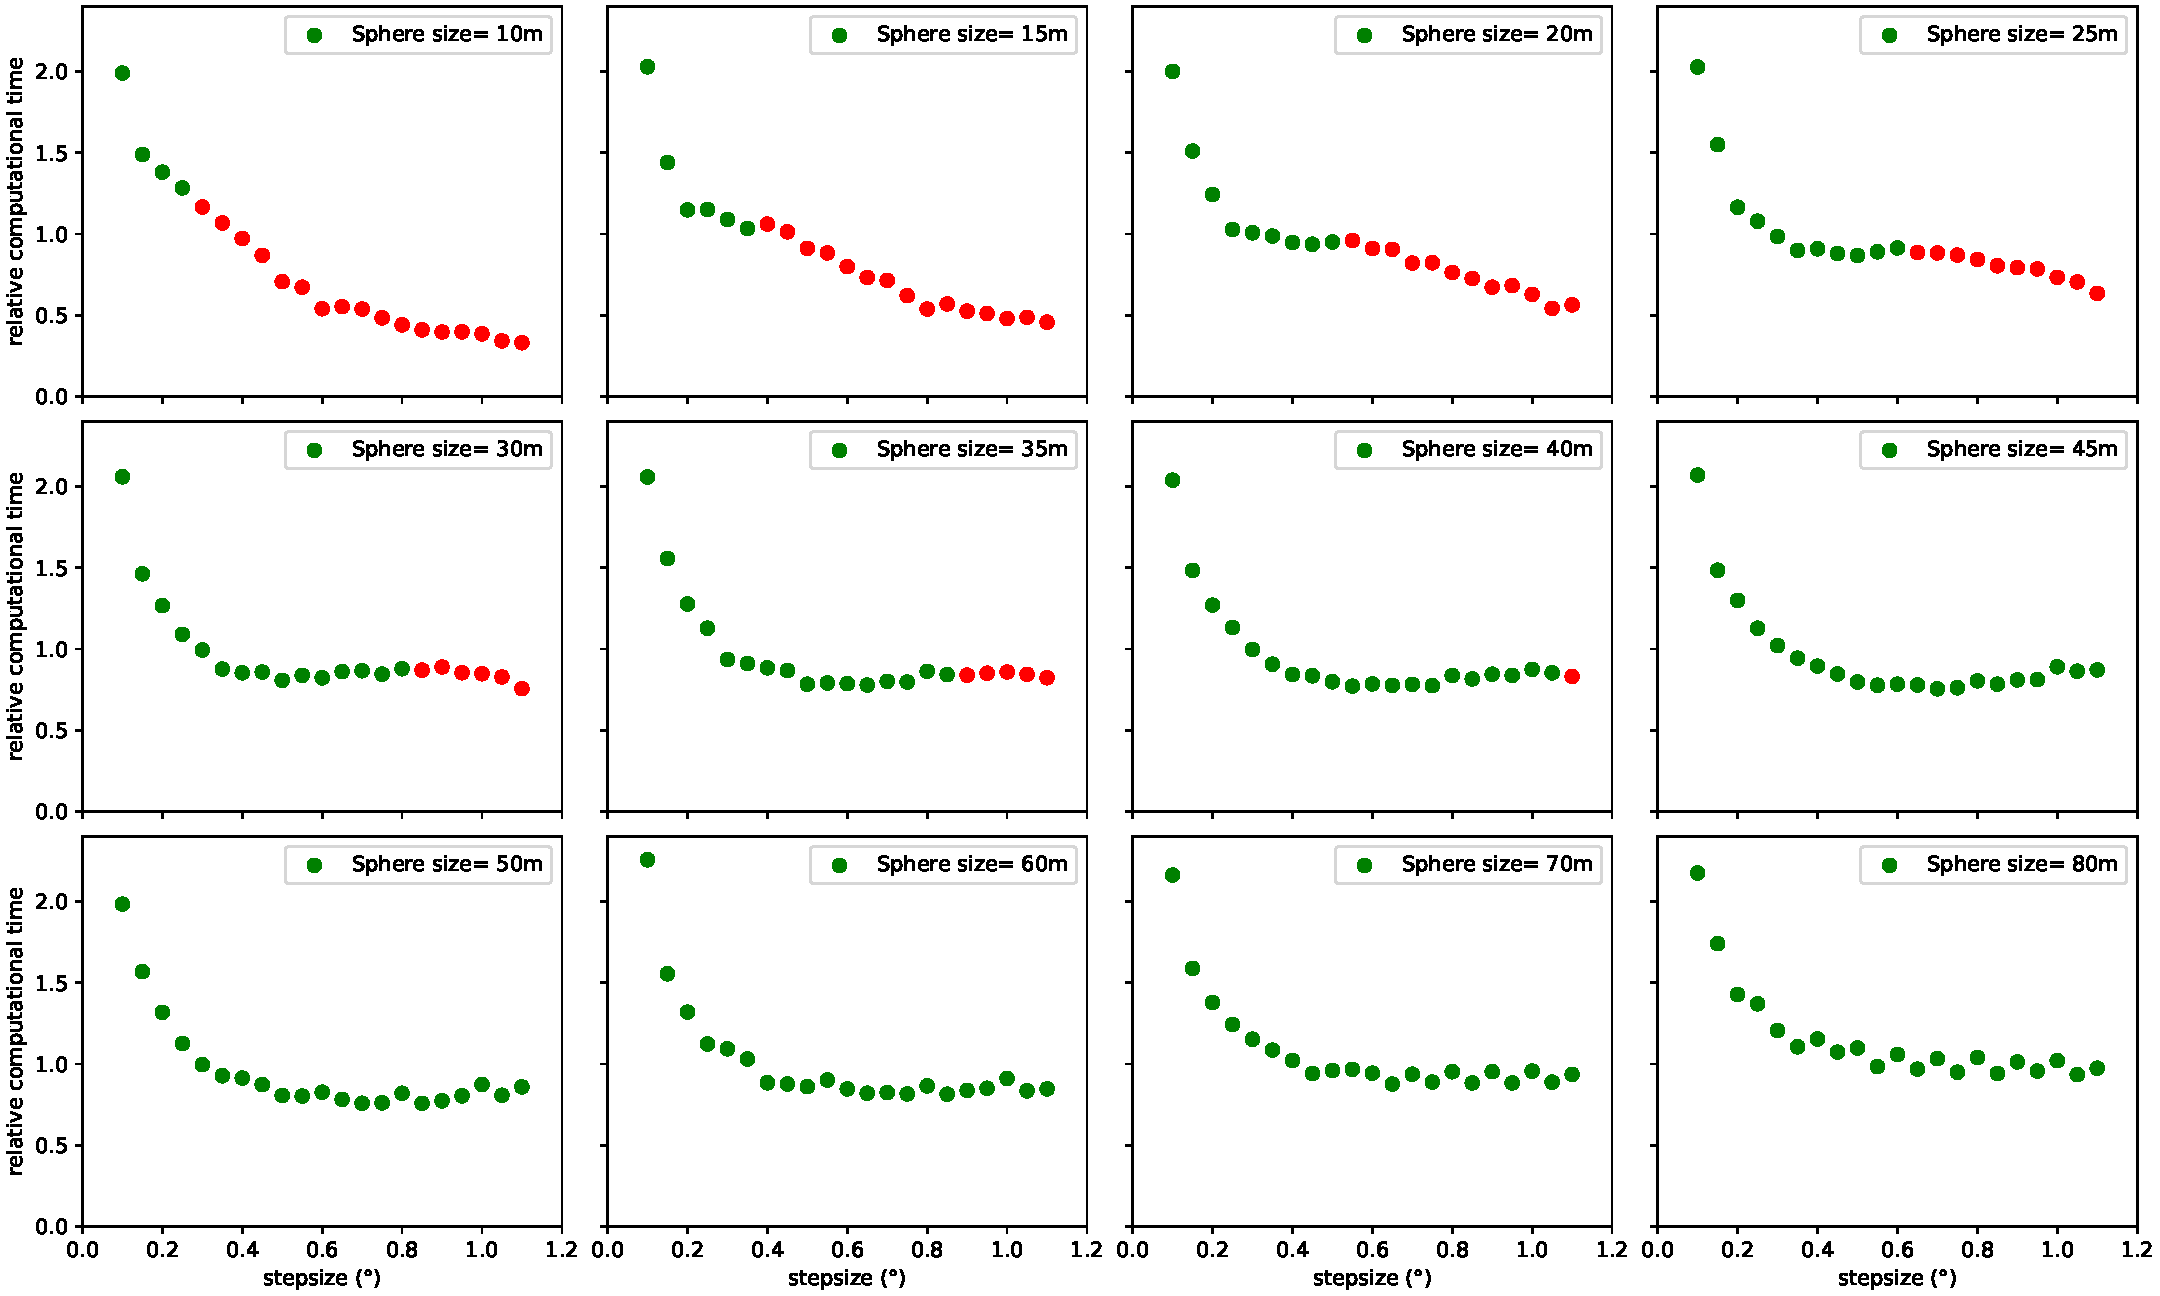
\includegraphics[width=\textwidth]{figures/subplotofallstepsphere.pdf}
	\caption{Variation in Sphere and angle step size with report on relative time.}
	\label{fig:SphereStepInfl}
\end{figure}

\begin{figure}
	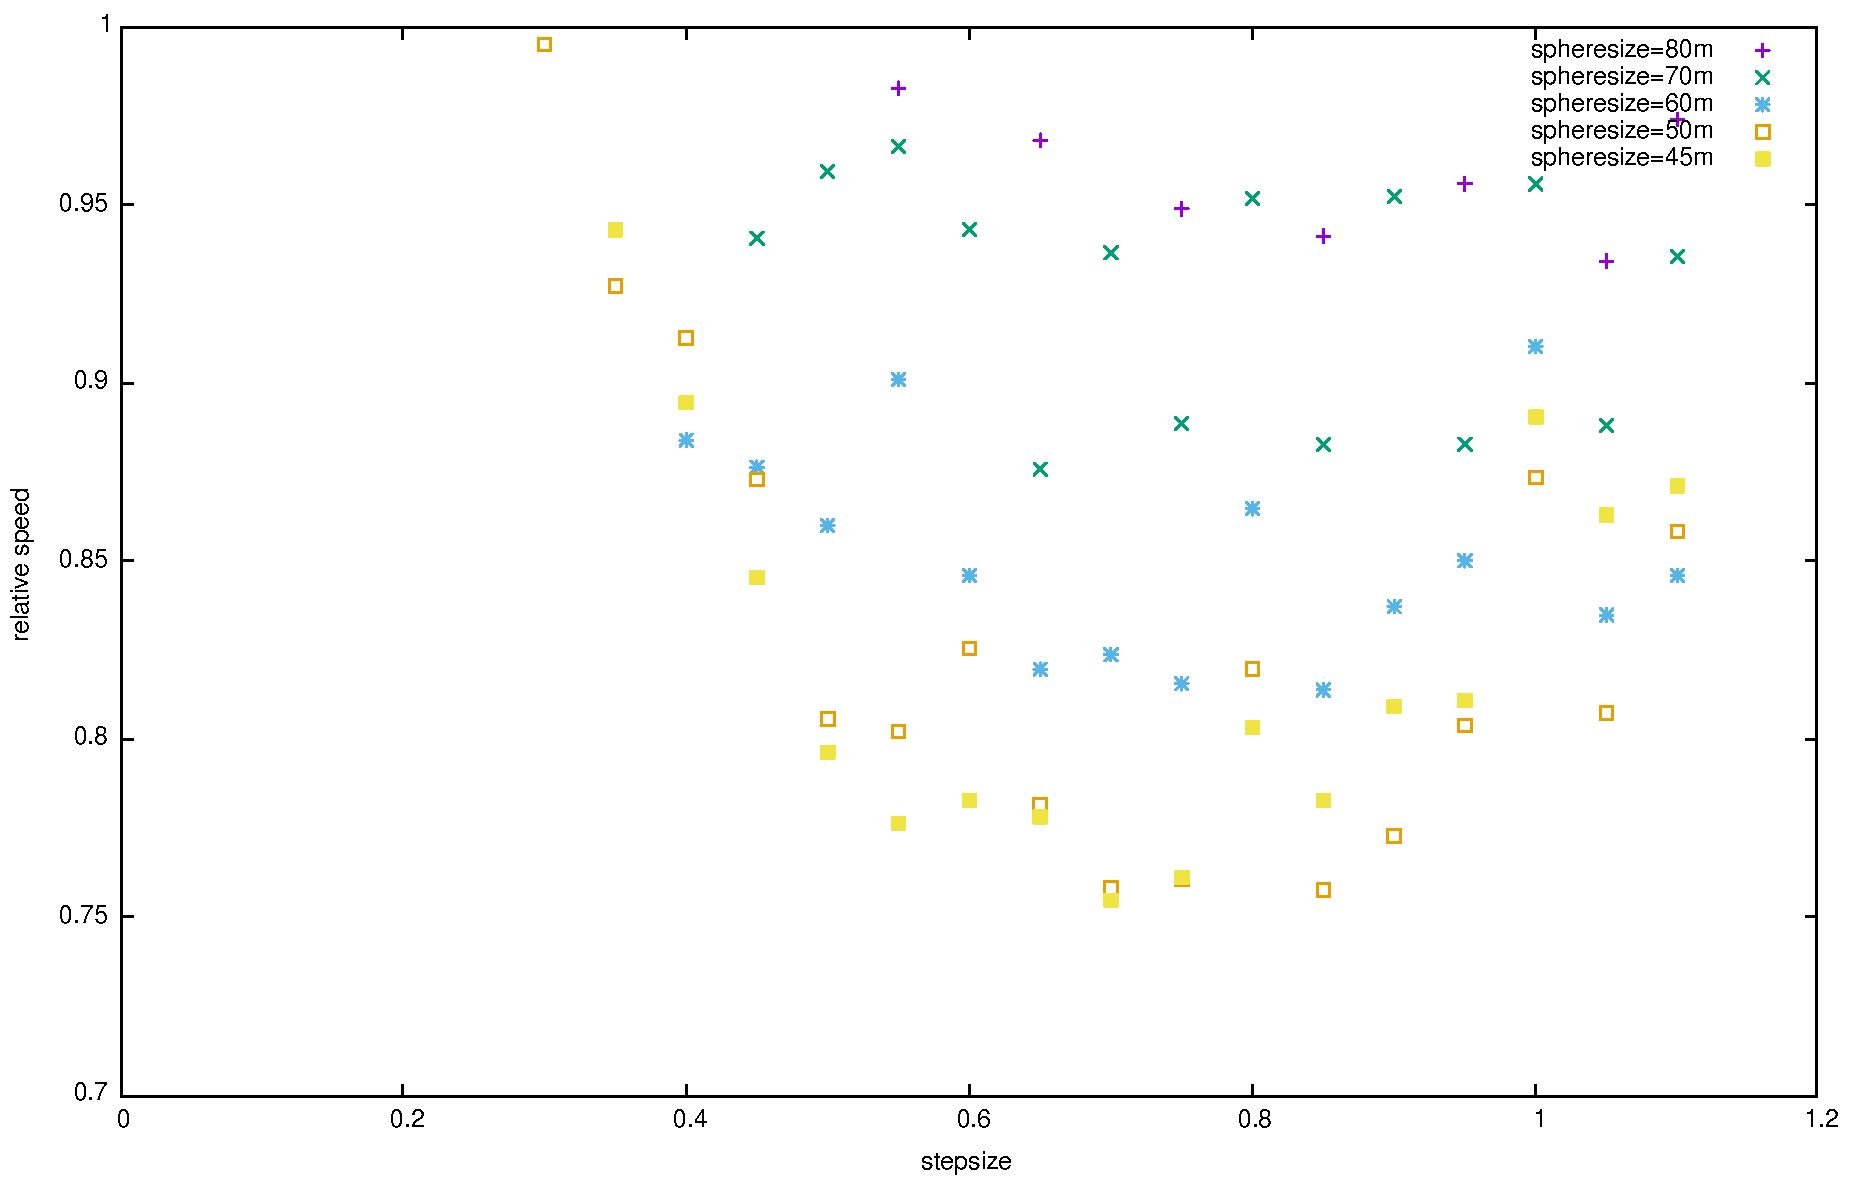
\includegraphics[width=\textwidth]{figures/SphereAndStepFinal.pdf}
	\caption{Green values in variation in sphere and angle step size with report on relative time.}
	\label{fig:SphereStepFinal}
\end{figure}

% =====================================================================
% End matter
% =====================================================================
\newpage
%----------------------------------------------------------------------------------------
%	REFERENCE LIST
%----------------------------------------------------------------------------------------
\bibliography{sources}
\bibliographystyle{plain}

\end{document}
